\documentclass[12pt, a4paper]{article}
\usepackage{amsfonts, amsmath, amssymb, amsthm}
\usepackage{enumitem}
\usepackage{mathtools}
\usepackage{fullpage}
\usepackage{mathrsfs}
\usepackage{float}
\usepackage{tikz-cd}
\usepackage{tikz}
\usepackage{quiver}


\theoremstyle{plain}
\newtheorem{innercustomgeneric}{\customgenericname}
\providecommand{\customgenericname}{}
\newcommand{\newcustomtheorem}[2]{%
\newenvironment{#1}[1]{
\renewcommand\customgenericname{#2}%
\renewcommand\theinnercustomgeneric{##1}%
\innercustomgeneric
}
{\endinnercustomgeneric}
}
\newcustomtheorem{lemma}{Lemma}

\makeatletter
\newcommand*\bigcdot{\mathpalette\bigcdot@{.5}}
\newcommand*\bigcdot@[2]{\mathbin{\vcenter{\hbox{\scalebox{#2}{$\m@th#1\bullet$}}}}}
\makeatother

\setcounter{section}{1}

\newcommand{\vertiii}[1]{{\left\vert\kern-0.25ex\left\vert\kern-0.25ex\left\vert #1 
    \right\vert\kern-0.25ex\right\vert\kern-0.25ex\right\vert}}
\makeatletter

\newcommand{\N}{\mathbb{N}}
\newcommand{\Hs}{\mathbb{H}}
\newcommand{\A}{\mathscr{A}}
\newcommand{\B}{\mathscr{B}}
\newcommand{\U}{\mathscr{U}}
\newcommand{\Q}{\mathbb{Q}}
\newcommand{\R}{\mathbb{R}}
\newcommand{\Z}{\mathbb{Z}}
\newcommand{\C}{\mathbb{C}}
\newcommand{\cC}{\mathsf{C}}
\newcommand{\Ab}{\mathsf{Ab}}
\newcommand{\Set}{\mathsf{Set}}
\newcommand{\Grp}{\mathsf{Grp}}



\newcommand{\set}[1]{\mathbb{#1}}
\newcommand{\F}{\mathcal{F}}
\newcommand{\T}{\mathcal{T}}
\newcommand{\G}{\mathcal{G}}
\newcommand{\Ps}{\mathscr{P}}
\newcommand{\card}{\mathbf{card}}
\DeclareMathOperator{\inter}{Int} 
\DeclareMathOperator{\Hom}{Hom}
\DeclareMathOperator{\lcm}{lcm}
\DeclareMathOperator{\Aut}{Aut}
\DeclareMathOperator{\Inn}{Inn}
\DeclareMathOperator{\Id}{Id}
\DeclareMathOperator{\Stab}{Stab}
\DeclareMathOperator{\Obj}{Obj}
\DeclareMathOperator{\coker}{coker}
\DeclareMathOperator{\Image}{Im}
\DeclareMathOperator{\O}{O}
\def\phi{\varphi}
\def\epsilon{\varepsilon}
\def\into{\hookrightarrow}




\usepackage{xcolor}
\usepackage{mdframed}
\usepackage{indentfirst}
\usepackage{hyperref}
\newenvironment{exercise}[2][Exercise]
    { \begin{mdframed}[backgroundcolor=gray!20] \textbf{#1 #2} \\}
    {  \end{mdframed}}
    
\newenvironment{problem}[2][Problem]
    { \begin{mdframed}[backgroundcolor=gray!20] \textbf{#1 #2} \\}
    {  \end{mdframed}}


\title{Answer to Algebra Chapter 0 by Paolo Aluffi}
\author{Hoang Vo Ke}
\date{\today}

\begin{document}
\maketitle

\section*{Chapter I. Preliminaries: Set theory and categories}
\subsection*{1.3. Categories}

\begin{exercise}{1}
Let $C$ be a category. Consider a structure $C^{op}$ with
\begin{itemize}
\item $\text{Obj}(C^{op}):=\text{Obj}(C)$;
\item for $A$, $B$ objects of $C^{op}$ (hence objects of $C$), $\text{Hom}_{C^{op}}(A,B) := \text{Hom}_C(B,A)$.
\end{itemize}
Show how to make this into a category (that is, define composition of morphisms in $C^{op}$ and verify the properties listed in 3.1.
\end{exercise}
	\begin{proof}
	For any $f\in \text{Hom}_{C^{op}}(A,B)$ and $g\in \text{Hom}_{C^{op}}(B,C)$, we define the composition $g\circ f$ of $C^{op}$ to be the composition $fg$ of $C$. (We will denote the composition in $C^{op}$ with "$\circ$" and nothing for the composition in $C$). With this definition, we have $$h\circ (g\circ f) = h\circ fg = (fg)h = f(gh) = f(h\circ g) = (h\circ g)\circ f,$$
	which says this composition law is associative.
	
	For any object $A$ of $C$, let the identity of $\text{Hom}_{C^{op}}(A,A)$ equals the identity of $\text{Hom}_{C}(A,A)$. So for any $f\in \text{Hom}_{C^{op}}(A,B) = \text{Hom}_{C}(B,A)$, we have $f\circ 1_A=1_Af = f$. Similarly, we get $1_B\circ f = f1_B=f$. So $C^{op}$ is a category.
	\end{proof}


\begin{exercise}{3}
Formulate precisely what it means to say that $1_a$ is an identity with respect to composition in Example 3.3, and prove this assertion.
\end{exercise}
	\begin{proof}
	To show that $1_A$ is an identity, we must show that for $f\in \text{Hom}(a,b)$, we have $1_bf = f = f1_a$. Indeed, we have $1_bf = (b,b)(a,b) = (a,b) = f$ and $f 1_a=(a,b)(a,a)=(a,b)=f$. So $1_a$ is an identity with respect to the composition in Example 3.3.
	\end{proof}
	
\pagebreak

\begin{exercise}{4}
Can we define a category in the style of Example 3.3 using the relation $<$ on the set $\Z$?
\end{exercise}
	\begin{proof}
	No we cannot define a category in style of Example 3.3 using the relation $<$ because it is not reflexive. Therefore, there is no identity morphism.
	\end{proof}

\begin{exercise}{5}
Explain in what sense Example 3.4 is an instance of the categories considered in Example 3.3
\end{exercise}
	\begin{proof}
	Because the $\subseteq$ relation is transitive and reflexive, we can define a category out of $P(S)$ similar to Example 3.3.
	\end{proof}

\begin{exercise}{7}
Define carefully objects and morphisms in Example 3.7, and draw the diagram corresponding to composition.
\end{exercise}
	\begin{proof}
	Let $C$ be a category, we will define $C_A$ as follow 
	\[
	\text{Obj}(C_A) = \{f:f\in \text{Hom}(A,B) \text{ for some }B\in \text{Obj}(C)\}.
	\]
	Let $f\in \text{Hom}_{C}(A,B)$, $g\in \text{Hom}_C(A,D)$, and $h\in \text{Hom}_{C}(A,E)$, then we will define the morphism $f\rightarrow g$ be the commutative diagram.
	\begin{center}
	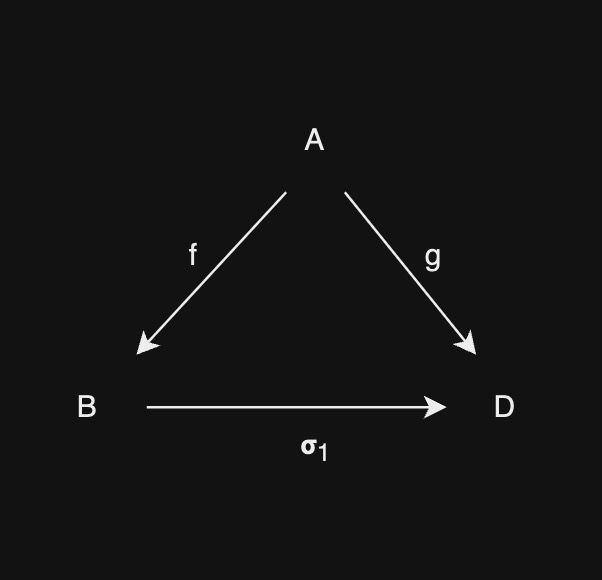
\includegraphics[scale=0.2]{1}
	\end{center}
The identity of $f$ would be this diagram.
\begin{center}
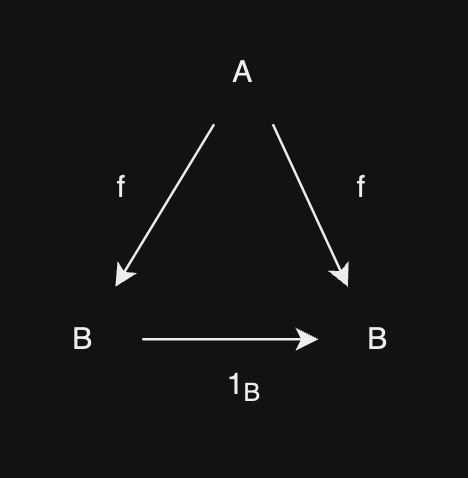
\includegraphics[scale=0.2]{2}
\end{center}
	Similar to Example 3.7, we can define the composition of two diagrams $f\rightarrow g$ and $g\rightarrow h$ as follow.
	\begin{center}
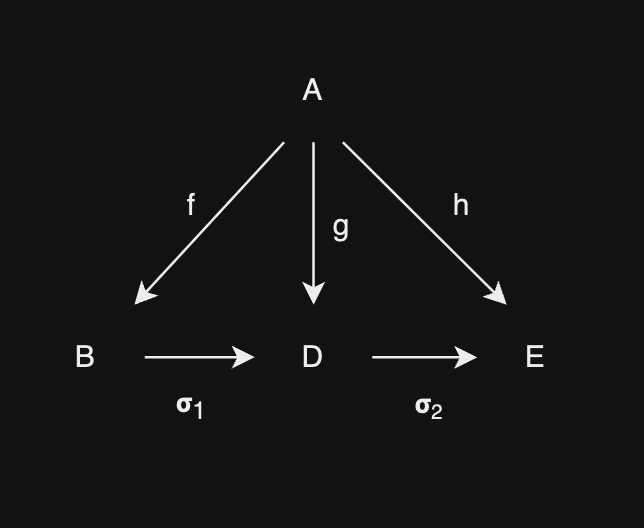
\includegraphics[scale=0.2]{3}
\end{center}
	Because $C$ is a Category, the previous diagram is the same as this.
	\begin{center}
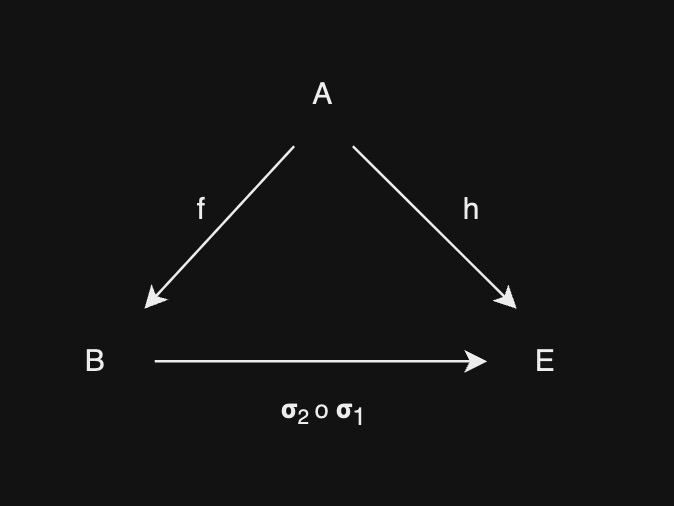
\includegraphics[scale=0.2]{4}
\end{center}
And it is not hard to check that is definition satisfies all the properties of a Category. (Trust me, I have done it on paper.)
	\end{proof}

\subsection*{4. Morphisms}
\begin{exercise}{4.3}
Let $A,B$ be objects of a category $C$, and let $f\in \Hom_C(A,B)$ be a morphism.
\begin{itemize}
\item Prove that if $f$ has a right-inverse, then $f$ is an epimorphism.
\item Show that the converse does not hold, by giving an explicit example of a category and an epimorphism without a right-inverse.
\end{itemize}
\end{exercise}
	\begin{proof}
\hfill	\begin{itemize}
	\item Assume that $f\in \Hom_C(A,B)$ has a right inverse, say $f'$, then $f\circ f'=1_A$. For any $\beta$ and $\beta'$ in $C$ such that $\beta\circ f = \beta' \circ f$, then we would have
	\[
	\beta = \beta \circ (f\circ f') = (\beta \circ f)\circ f' = (\beta'\circ f)\circ f' = \beta'.
	\]
	So $f$ is an epimorphism.
	\item The converse is not true however. Take the category $\Z$ with the relation $\leq$ as an example. Any morphism is an epimorphism but $(3,5)$ doesn't have an inverse.
	\end{itemize}
	\end{proof}
	
	
\subsection*{5. Universal properties}

\begin{exercise}{5.1}
Prove that a final object in a category $C$ is initial in the opposite category $C^{op}$.	
\end{exercise}
	\begin{proof}
	Let $A$ be a final object of $C$, so for any $B\in C$, we have $\Hom_{C^{op}}(A,B)=\Hom_C(B,A)$ is a singleton. So $A$ is an initial object in $C^{op}$.
	\end{proof}


\begin{exercise}{5.2}
Prove that $\varnothing$ is the unique initial object in $Set$.
\end{exercise}
	\begin{proof}
	Let $A\neq \varnothing$ be an initial object in Set. Let $\{x,y\}\in Set$ be an object of $Set$ that has two elements. We can define two distinct functions in $\Hom(A,\{x,y\})$, namely $f(a)=x$ and $f(a)=y$ for all $a\in A$. But this is impossible since $A$ is an initial object, thus $\varnothing$ is the unique initial object of $Set$.
	\end{proof}

\begin{exercise}{5.3}
Prove that final objects are unique up to isomorphism.
\end{exercise}
	\begin{proof}
	Let $A$ and $B$ be two final objects of a category $C$. Notice that the unique element of $\Hom(A,A)$ is $1_A$ and the same for $B$. Let $f\in \Hom(A,B)$ and $g\in \Hom(B,A)$. Then $f\circ g\in \Hom(B,B)$, which implies $f\circ g = 1_B$. Similarly we get $g\circ f = 1_A$. So $A$ is isomorphic to $B$.
	\end{proof}


\begin{exercise}{5.6}
Consider the category corresponding to endowing (as in Example 3.3) the set $\Z^+$ of positive integers with the divisibility relation. Thus there is exactly one morphism $d\to m$ in this category if and only if $d$ divides $m$ without remainder; there is no morphism between $d$ and $m$ otherwise. Show that this category has products and coproducts. What are their "conventional" names?
\end{exercise}
    \begin{proof}
        Let $a,b\in \Z^+$, we will show that $d = \gcd(a,b)$ is the product and $m = \lcm(a,b)$ is the coproduct of $a$ and $b$. Indeed, because $d|a$ and $d|b$, we get $d\to a$ and $d\to b$. For any $c\to a$ and $c\to b$, we get $c|a$ and $c|b$. Therefore $c|\gcd(a,b)=d$. Hence there is a unique morphism $c\to d$. So $d$ is the product of $a$ and $b$. Similarly, we can show that $m = \lcm(a,b)$ is the coproduct of $a$ and $b$. 
    \end{proof}

\pagebreak

\begin{exercise}{5.8}
Show that in every category $C$ the products $A\times B$ and $B\times A$ are isomorphic if they exist.
\end{exercise}
    \begin{proof}
        Let $\pi_A,\pi_B$ be the natural projection from $B\times A$ to $A$ and $B$ respectively. Similarly, let $\pi_A'$ and $\pi_B'$ be the natural projection from $A\times B$ to $A$ and $B$. Because $A\times B$ and $B\times A$ are products, there is a unique $f\in\Hom(A\times B,B\times A)$ and $g\in \Hom(B\times A,A\times B)$ such that 1 commute.
        \begin{figure}[H]
            \centering
            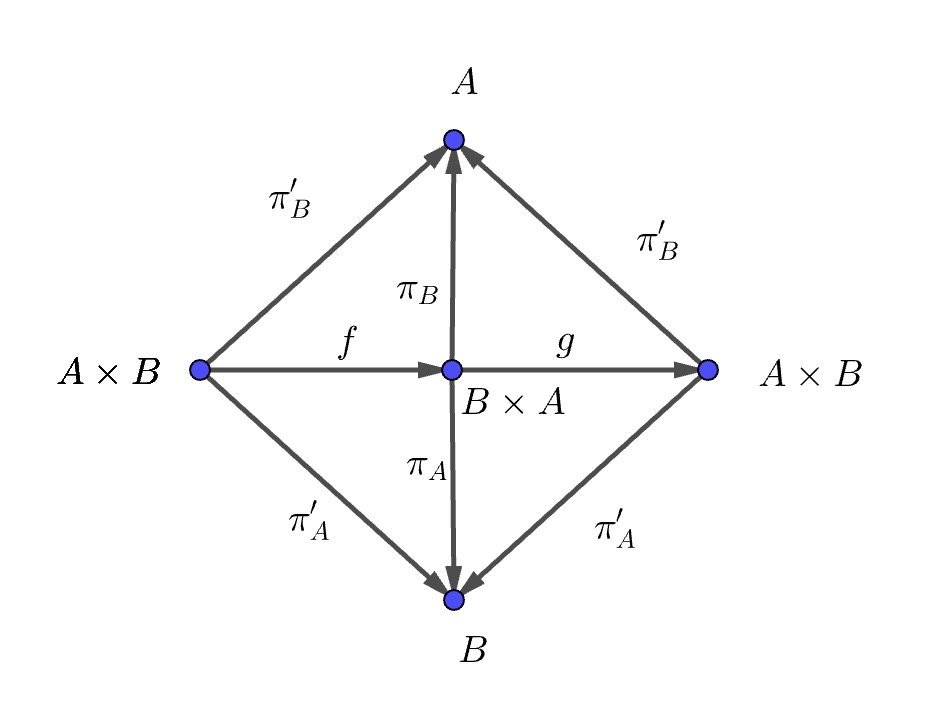
\includegraphics[scale = 0.3]{Aluffi/5.jpg}
            \caption{diagram 1}
            \label{fig:1}
        \end{figure}
        But diagram 1 can be reduced to diagram 2. We can see that by replacing $f\circ g$ by $1_{A\times B}$, the diagram also commute. Using the universal property of the product, we get $f\circ g =1_{B\times A}$. 
        \begin{figure}[H]
            \centering
            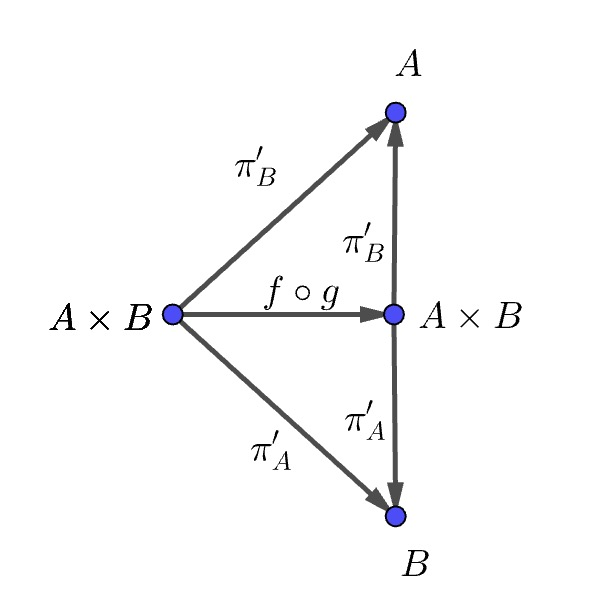
\includegraphics[scale = 0.3]{Aluffi/6.jpg}
            \caption{diagram 2}
            \label{fig:2}
        \end{figure}
        Similarly, we can show that $g\circ f = 1_{A\times B}$. So $A\times B$ and $B\times A$ are isomorphic.
    \end{proof}


\begin{exercise}{5.10}
Push the envelope a little further still, and define products and coproducts for families (i.e., indexed sets) of objects of a category.\\
Do these exist in Set?\\
It is common to denote the product $A\times A\times\cdots\times A$ by $A^n$.
\end{exercise}

\section*{Chapter II. Groups, first encounter}

\subsection*{1. Definition of Group.}

\begin{exercise}{1.3}
    Prove that $(gh)^{-1}=h^{-1}g^{-1}$ for all elements $g,h$ of a group $G$.
\end{exercise}
    \begin{proof}
        By considering each element of a group as a morphism, Proposition 4.3 yields the result immediately.
    \end{proof}

\begin{exercise}{1.5}
    Prove that every column of the multiplication table of a group contains all elements of the group exactly once.
\end{exercise}
    \begin{proof}
        Each row of the multiplication table is the image of a group $G$ through an isomorphism $f$. The epimorphism of $f$ guarantees each column contains all elements of $G$, and the monomorphism guarantees each element appears exactly once.  
    \end{proof}

\begin{exercise}{1.6}
    Prove that there is only one possible multiplication table for $G$ if $G$ has exactly $1,2,$ or $3$ elements. Analyze the possible multiplication tables for groups with exactly $4$ elements, and show that there are two distinct tables, up to reordering the elements of $G$. Use these tables to prove that all groups with $\leq 4$ elements are commutative.
\end{exercise}
    \begin{proof}
        If $G$ has one or two elements, then $\Hom(G)$ has $1!$ or $2!$ elements respectively. So $G$ has one multiplication table. Assume that $G=\{e,g,h\}$. Notice that if $gh=g$, then the cancellation law implies $h=e$. Thus $gh=hg=e$. Fill in the table using Exercise 1.5, we get the following unique table.
            \begin{center}
                \begin{tabular}{c|ccc}
                 $\bigcdot$ & e & g & h \\
                 \hline
                 e & e & g& h\\
                 g & g & h & e\\
                 h & h & e & g
            \end{tabular}.
            \end{center}
        After a lot of checking, there are two distinct tables up to reordering as follows

        \begin{tabular}{c|cccc}
            $\bigcdot$ & e&g&h&k \\
            \hline
            e&e&g&h&k\\
            g&g&e&k&h\\
            h&h&k&g&e\\
            k&k&h&e&g
        \end{tabular},
        \quad and \quad
        \begin{tabular}{c|cccc}
            $\bigcdot$ & e&g&h&k \\
            \hline
            e&e&g&h&k\\
            g&g&e&k&h\\
            h&h&k&e&g\\
            k&k&h&g&e
        \end{tabular}. 

        Since all of these tables are symmetric with respect to the main diagonal, groups with less than 4 elements are commutative.
    \end{proof}

\begin{exercise}{1.7}
    Prove Corollary 1.11, that is $g^N=e$ if and only if $N$ is a multiple of $|g|$ for an element $g$ of finite order, and $N\in\Z$. 
\end{exercise}
    \begin{proof}
        Let $r$ be the reminder when we divide $N$ by $|g|$. So $r<|g|$. Clearly, we get $g^r=e$. Since $|g|$ is the least nonzero number that satisfies this equation, we get $r=0$. So $N$ is a multiple of $|g|$.
    \end{proof}

\begin{exercise}{1.11}
    Prove that for all $g,h$ in a group $G$, $|gh|=|hg|$. 
\end{exercise}
    \begin{proof}
        It is sufficient to prove that for any $n\in \N$, $(gh)^n=e$ implies $(hg)^n=e$. Indeed, because if $(gh)^n=e$, then
        \[
        e = heh^{-1} = h(gh)^nh^{-1}=(hg)^n.
        \]
        So $|gh|=|hg|$.
    \end{proof}


\subsection*{2. Examples of Group.}

\begin{exercise}{2.1}
    Prove that, with this notation,
    \[
    M_{\sigma\tau} = M_\sigma M_\tau
    \]
    for all $\sigma,\tau \in S_n$, where the product on the right is the ordinary product of matrices. 
\end{exercise}
    \begin{proof}
        Let $M(i,j)$ be the entry at $(i,j)$ of a matrix $M$.
        Because $\sigma$ is an isomorphism, each row and column of $M_\sigma$ has exactly one $1$. Let $M_{\sigma\tau} := M_\sigma M_\tau$, we have
        \[
        M_{\sigma \tau}(i,j)=\sum_{t=1}^{n}{M_\sigma(i,t)M_\tau(t,j)}.
        \]
        Notice that there is only one $t$ that makes $M_\sigma(i,t)\neq 0$, so $M_{\sigma \tau}(i,j)=1$ if and only if $M_\sigma(i,t)=M_\tau(t,j)=1$. This means $t = \sigma(i)$ and $j=\tau(t)=\tau(\sigma(i))$. So $M_{\sigma\tau}$ the matrix represent the permutation $\sigma\tau$.
    \end{proof}

\begin{exercise}{2.4}
    Define a homomorphism $D_8\to S_4$ by labeling the vertices of a square, as we did for a triangle in $\S 2.2$. List the $8$ permutations in the image of this homomorphism.
\end{exercise}
    \begin{proof}
        We know that $D_8=\langle{r,s\mid r^4=s^2=e, rs=sr^{-1}}\rangle$. Define $f:D_8\to S_4$ that maps 
        \[
        e\mapsto e, \quad r\mapsto (1234),\quad s\mapsto (24).
        \]
        With brute force, we can check that $(1234)^4=(24)^2=e$ and $(1234)(24)=(24)(1234)^{-1}$. So $f$ is a homomorphism. The $8$ permutations in the image of $f$ are $$\{e,(1234),(13)(24),(1432),(13),(24),(12)(34),(14)(23)\}.$$ Since $D_8$ also has $8$ elements and it is not hard to check that $f$ is surjective, we get $f$ is an isomorphism.
    \end{proof}

\begin{exercise}{2.7}
    Find all elements of $D_{2n}$ that commute with every other elements.
\end{exercise}
    \begin{proof}
        We know that $$D_{2n}=\langle{r,s\mid r^n=s^2=e, rs=sr^{-1}}\rangle = \{e,r,\cdots,r^{n-1},s,rs,\cdots,r^{n-1}s\}.$$
        Clearly, $e$ commutes with every element, If $r^js$ commutes with every element, then it must commute with $r$. So 
        \[
        r^js = r^{j+1}sr^{-1} = r^jsr^{-2}.
        \]
        This implies $r^2=e$ or $n=2$, which is impossible because $n\geq 3$.

        If $r^j$ commutes with every element for some $j$ from $1$ to $n-1$, then it must commute with $s$. Thus
        \[
        r^j = sr^js = r^{-j}.
        \]
        This means $r^{2j} = 2$ or $j=n/2$. So $n$ must be an even number, say $n=2k$, and $r^k$ commutes with every element of $D_{2n}$. But this is not hard to check, using the formula $rs=sr^{-1}$. So when $n$ is even, there are exactly two elements, those are $e$ and $r^{n/2}$. Otherwise, $e$ is the only element that commute with everyone.
    \end{proof}


\subsection*{3. The category $\Grp$}


\begin{exercise}{3.1}
Let $\varphi\colon G\to H$ be a morphism in a category $C$ with products. Explain why there is a unique morphism
\[
(\varphi\times\varphi)\colon G\times G\to H\times H.
\]
(This morphism is defined explicitely for $\cC=\Set$ in $\S 3.1.$)
\end{exercise}
    \begin{proof}
        Let $\pi_G\colon G\times G\to G$ be the projection with respect to the first entry and $\pi'_G\colon G\times G\to G$ be the projection with respect to the second entry. Similar for $H$. Because $\pi_G\circ \varphi$ and $\pi'_G\circ\varphi$ are morphisms of $\cC$, the unniversal property of product implies that there exists a unique map $\varphi\times\varphi$ such that the following diagram commutes:
        \begin{figure}[H]
            \centering
            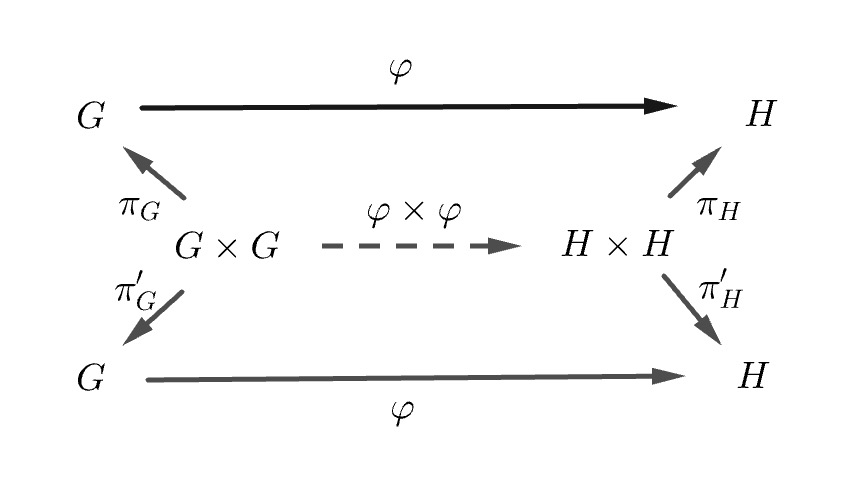
\includegraphics[scale=0.3]{Aluffi/7.jpg}
        \end{figure}
    \end{proof}


\begin{exercise}{3.2}
    Let $\varphi\colon G\to H,\psi\colon H\to K$ be morphisms in a category with products, and consider morphisms between the products $G\times G,H\times H,K\times K$ as in Exercise 3.1. Prove that 
    \[
    (\psi\varphi)\times (\psi\varphi) = (\psi\times \psi)(\varphi\times \varphi).
    \]
    (This is part of the commutative of the diagram displayed in $\S 3.2$.)
\end{exercise}
    \begin{proof}
        For any $(g_1,g_2)\in G\times G$, we have
        \begin{align*}
        ((\psi\varphi)\times (\psi\varphi))(g_1,g_2) &= (\psi\varphi(g_1))\times (\psi\varphi(g_2))\\
        &= (\psi\times\psi)(\varphi(g_1),\varphi(g_2))\\
        &= (\psi\times\psi)(\varphi\times\varphi)(g_1,g_2).
        \end{align*}
        This computation prove the required statement.
    \end{proof}


\begin{exercise}{3.3}
    Show that if $G,H$ are abelian groups, then $G\times H$ satisfies the universal property for coproducts in $\Ab$.
\end{exercise}
    \begin{proof}
        Let $G\times H$ be the group product of $G$ and $H$. Let $i_G\colon G\to G\times H$ maps $g\mapsto (g,e_H)$ and $i_H\colon H\to G\times H$ maps $h\to (e_G,h)$. Notice that $i_G$ is a homomorphism because for any $g_1,g_2\in G$, we have
        \[
        i_G(g_1\cdot g_2) = (g_1 \cdot g_2,e_H)=(g_1,e_H)\cdot (g_2,e_H) = i_G(g_1)\cdot i_G(g_2).
        \]
        Similarly, $i_H$ is a homomorphism.
        \begin{center}
            \begin{tikzcd}      
  &  &                                 & G \arrow[llld, "\varphi", bend right] \arrow[ld, "i_G"] \\
K &  & G\times H \arrow[ll, "\sigma"'] &                                                         \\
  &  &                                 & H \arrow[lllu, "\psi"', bend left] \arrow[lu, "i_H"]   
\end{tikzcd}
        \end{center}
        

    Let $\varphi$ and $\psi$ be homomorphism from $G$ and $H$ to $K$ respectively, we will show that there exists a unique homomorphism $\sigma$ such that the diagram above commutes. Indeed, assume that that diagram commute, then for any $(g,h)\in G\times H$, we get
    \begin{align*}
        \sigma(g,h) &= \sigma((g,e_H)\cdot(e_G,h))\\
        &=\sigma(g,e_H)\cdot \sigma(e_G,h)\\
        &=\sigma\circ i_G(g)\cdot \sigma\circ i_H(h)\\
        &=\varphi(g)\cdot \psi(h).
    \end{align*}
    Here, the first equality by the operation on $G\times H$, the second equality is because $\sigma$ is a homomorphism, and the last equality is because this diagram commutes. So if $\sigma$ exists, it is unique and $\sigma(g,h)=\varphi(g)\cdot\psi(h)$. Let $\sigma(g,h):=\varphi(g)\cdot\psi(h)$, we show that $\sigma$ is a homomorphism. Indeed, for $(g_1,h_1),(g_2,h_2)\in G\times H$, we have
    \[
    \sigma((g_1,h_1)\cdot (g_2,h_2))=\sigma(g_1g_2,h_1h_2) = \varphi(g_1)\varphi(g_2)\psi(h_1)\psi(h_2).
    \]
    But $K$ is commutative, thus the previous equation becomes
    \[
    \varphi(g_1)\psi(h_1)\varphi(g_2)\psi(h_2) = \sigma(g_1,h_1)\cdot\sigma(g_2,h_2).
    \]
    So $\sigma$ is a homomorphism, which complete our proof.
    \end{proof}

\begin{exercise}{3.6}
    Consider the product of the cyclic groups $C_2,C_3\colon C_2\times C_3$. By Exercise 3.3, this group is a coproduct of $C_2$ and $C_3$ in $\Ab$. Show that it is not a coproduct of $C_2$ and $C_3$ in $\Grp$, as follow:
    \begin{itemize}
        \item find injective homomorphisms $C_2\to S_3$, $C_3\to S_3$;
        \item arguing by contradiction, assume that $C_2\times C_3$ is a coproduct of $C_2,C_3$, and deduce that there would be a group homomorphism $C_2\times C_3\to S_3$ with certain properties;
        \item show that there is no such homomorphism.
    \end{itemize}
\end{exercise}
    \begin{proof}
        Let $\varphi_1\colon C_2\to \{e,(1,2)\}$ and $\varphi_2\colon C_3\to \{e,(123),(132)\}$ be isomorphisms. Assume that $C_2\times C_3$ is a coproduct of $C_2$ and $C_3$, then there exists a $\sigma\colon C_2\times C_3\to S_3$ that makes the diagram 
        \begin{center}
            % https://q.uiver.app/#q=WzAsNCxbMCwxLCJTXzMiXSxbMiwxLCJDXzJcXHRpbWVzIENfMyJdLFszLDAsIkNfMiJdLFszLDIsIkNfMyJdLFsxLDAsIlxcc2lnbWEiLDJdLFsyLDEsImlfMSIsMl0sWzMsMSwiaV8yIiwyXSxbMywwLCJcXHZhcnBoaV8yIiwwLHsiY3VydmUiOi0yfV0sWzIsMCwiXFx2YXJwaGlfMSIsMix7ImN1cnZlIjoyfV1d
\begin{tikzcd}
	&&& {C_2} \\
	{S_3} && {C_2\times C_3} \\
	&&& {C_3}
	\arrow["\sigma"', from=2-3, to=2-1]
	\arrow["{i_1}"', from=1-4, to=2-3]
	\arrow["{i_2}"', from=3-4, to=2-3]
	\arrow["{\varphi_2}", curve={height=-12pt}, from=3-4, to=2-1]
	\arrow["{\varphi_1}"', curve={height=12pt}, from=1-4, to=2-1]
\end{tikzcd}
        \end{center}
        commutes. So the image of $\sigma$ must contain $\{e,(1,2),(123),(132)\}$. Since the image of $\sigma$ is a subgroup, it equals $S_3$. But this is impossible because $C_2\times C_3$ is abelian, whereas $S_3$ is not. So $\sigma$ does not exist.
    \end{proof}


\subsection*{4. Group homomorphisms}

\begin{exercise}{4.3}
    Prove that a group of order $n$ is isomorphic to $\Z/n\Z$ if and only if it contains an element of order $n$.
\end{exercise}
    \begin{proof}
        Let $G$ be a group of order $n$. If $\varphi\colon G\to \Z/n\Z$ is an isomorphism, then $\varphi^{-1}(1)$ has order $n$ by Proposition 4.8. Conversely, if $g\in G$ is an element of order $n$, then $G$ is a cyclic group generated by $n$. But any cyclic group of order $n$ is isomorphic to $\Z/n\Z$, thus we have the conclusion.
    \end{proof}


\begin{exercise}{4.5}
    Prove that the groups $(\R\setminus \{0\},\cdot)$ and $(\C\setminus \{0\},\cdot)$ are not isomorphic.
\end{exercise}
    \begin{proof}
        These sets are not isomorphic because $i\in \C\setminus\{0\}$ has order $4$, where there is no order $4$ element of $\R\setminus \{0\}$.
    \end{proof}


\begin{exercise}{4.8}
    Let $G$ be a group, and let $g\in G$. Prove that the function $\gamma_g\colon G\to G$ defined by $(\forall a\in G):\gamma_g(a) = gag^{-1}$ is an automorphism of $G$. Prove that the function $G\to \Aut(G)$ defined by $g\mapsto \gamma_g$ is a homomorphism. Prove that this homomorphism is trivial if and only if $G$ is abelian.
\end{exercise}
    \begin{proof}
        For the first part, it is sufficient to show that $\gamma_g$ is a homomorphism. Indeed, for any $a,b\in G$, we have
        \[
        \gamma_g(a)\gamma_g(b) = (gag^{-1})(gbg^{-1}) = gabg^{-1} = \gamma_g(ab).
        \]
        For the second part, let $g,h\in G$, then
        \[
        gh\mapsto \gamma_{gh}.
        \]
        But for any $a\in G$, we have 
        \[
        \gamma_{gh}=ghah^{-1}g^{-1} = g\gamma_h(a)g^{-1} = \gamma_g\circ\gamma_h(a).
        \]
        Thus $\gamma_{gh} = \gamma_g\circ \gamma_h$, which prove that the function defined by $g\mapsto \gamma_g$ is a homomorphism.
        For the third part, if $G$ is abelian, then $\gamma_g(a) = gag^{-1} = gg^{-1}a=a$. Thus $g\mapsto \gamma_g=\Id_{G}$ for all $g\in G$, which is the trivial homomorphism. Conversely, if $g\mapsto\gamma_g$ is trivial, then $\gamma_g(a) = a$ for all for any $g,a\in G$. But this implies that $ga=ag$ for any $a,g\in G$, thus $G$ is abelian.
    \end{proof}


\begin{exercise}{4.9}
    Prove that if $m,n$ are positive integers such that $\gcd(m,n)=1$, then $C_{mn}\cong C_m\times C_n$.
\end{exercise}
    \begin{proof}
        Let $d$ be the order of $e\in C_{m}\times C_n$, it is sufficient to show that $d = mn$. Because there is a natural homomorphism projection from $C_m\times C_n$ to $C_m$ and $e_m\in C_m$ has order $m$, we get $m|d$. Similarly, we get $n|d$. But $(m,n)=1$, thus $mn|d$, or $mn\leq d$ (this is because $d>0$). But $C_{m}\times C_n$ has $mn$ elements, thus $d\leq mn$. So $d=mn$, which complete our proof. 
    \end{proof}

\pagebreak

\begin{exercise}{4.10}
    Let $p\neq q$ be odd prime integers; show that $(\Z/pq\Z)^*$ is not cyclic.
\end{exercise}
    \begin{proof}
        Let us recall that 
        \[
        (\Z/n\Z)^*:=\{[m]_n\in \Z/n\Z\mid \gcd(m,n)=1\}.
        \]
        One can easily see that the order of $(\Z/pq\Z)^*$ is $\phi(pq)=(p-1)(q-1)$, where $\phi$ is the Euler function. Assume that $(\Z/pq\Z)^*$ is cyclic and is generated by $t$, then $t^{(p-1)(q-1)/2}$ is the only element that has order $2$. We will show that $(\Z/pq\Z)^*$ has at least 2 order-2 elements, thus contradicting to the cyclic hypothesis. 
        
         To find the first element, we consider the isomorphism $\varphi\colon \Z/pq\Z\to \Z/p\Z\times \Z/q\Z$ that maps $[x]_{pq}\mapsto ([x]_p,[x]_q)$. We will claim that $a = \varphi^{-1}([1]_p,[-1]_q)$ has order $2$. Indeed, $[a]_p=[1]_p$ implies $[a]_p^2=[1]_p$ and $[a]_q^2=[-1]_q^2=[1]_q$. So $\varphi(a^2)=([1]_p,[1]_q)$. But $\varphi([1]_{pq})=([1]_p,[1]_q)$, the "bijectiveness" of $\varphi$ implies that $a^2 = [1]_{pq}$. Clearly $a\neq [1]_{pq}$ because $\varphi([1]_{pq})=([1]_p,[1]_q)$, we claim that $a$ has order $2$.

         Similarly, we can point out that the second element is $b = \varphi^{-1}([-1]_p,[1]_q)$. Notice that $a\neq b$ because $p,q>2$, thus $[1]_p\neq [-1]_p$ and similar for $q$.
    \end{proof}


\begin{exercise}{4.11}
    In due time we will prove the easy fact that if $p$ is a prime integer, then the equation $x^d=1$ can have at most $d$ solutions in $\Z/p\Z$. Assume this fact, and prove that the multiplicative group $G=(\Z/p\Z)^*$ is cyclic.
\end{exercise}
    \begin{proof}
    Let $g\in G$ be the element of maximal order. Because $G$ is commutative, Exercise 1.15 implies that $h^{|g|}=1$ for all $h\in G$. It is not hard to check that $|G|=p-1$, thus the equation $x^{|g|}$ has $p-1$ zeros. By our hypothesis, $p-1\leq |g|$. Thus $|g|=p-1$ and $g$ is the element that generates $G$.
    \end{proof}


\begin{exercise}{4.14}
    Prove that the order of the group of automorphisms of a cyclic group $C_n$ is the number of positive integers $r<n$ that are relatively prime to $n$.
\end{exercise}
    \begin{proof}
        Let $C_n=\langle a\rangle$ be an arbitrary cyclic group. Any isomorphism $\varphi\colon C_n\to C_n$ is determined by where $a$ is mapped to. Notice that $\varphi$ is a homomorphism implies that $|\varphi(a)| \mid |a| = n$ and $\varphi^{-1}$ homomorphic implies that $n\mid|\varphi(a)|$. So $|\varphi(a)|=n$. But $a^r$ has order $n$ if and only if $\gcd(r,n)=1$, so the number of automorphism of $C_n$ equals the number of $r$ such that $\gcd(r,n)=1$.
    \end{proof}


\begin{exercise}{4.18}
    Prove the second part of Proposition 4.8. That is, let $\varphi\colon G\to H$ be an isomorphism. Show that $G$ is commutative if and only if $H$ is commutative.
\end{exercise}
    \begin{proof}
        For any $h_1,h_2\in H$, the isomorphic of $\varphi$ implies that there exists $g_1,g_2\in G$ such that $\varphi(g_1)=h_1$ and $\varphi(g_2)=h_2$. So
        \[
        h_1h_2 = \varphi(g_1)\varphi(g_2) = \varphi(g_1g_2)=\varphi(g_2g_1)=\varphi(g_2)\varphi(g_1)=h_2h_1.
        \]
        Therefore, $H$ is commutative.
    \end{proof}


\subsection*{5. Free Group}

\begin{exercise}{5.3}
    Use the universal property of free groups to prove that the map $j\colon A\to F(A)$ is injective, for all sets $A$.
\end{exercise}
    \begin{proof}
        For any $a,b\in A$ such that $j(a)=j(b)$, we define $G=\Z/2\Z$ and $f\colon A\to G$ as follow:
        \[
        f(t) = \begin{cases}
            0 & t\neq b,\\
            1 & t = b.
        \end{cases}
        \]
        The universal property of free group implies the existence of a homomorphism $\sigma\colon F(A)\to G$ such that the diagram below commutes.
        % https://q.uiver.app/#q=WzAsMyxbMCwxLCJBIl0sWzAsMCwiRihBKSJdLFsxLDAsIkciXSxbMCwxLCJqIl0sWzAsMiwiZiIsMl0sWzEsMiwiXFxzaWdtYSJdXQ==
\[\begin{tikzcd}
	{F(A)} & G \\
	A
	\arrow["j", from=2-1, to=1-1]
	\arrow["f"', from=2-1, to=1-2]
	\arrow["\sigma", from=1-1, to=1-2]
\end{tikzcd}\]
        But this means $f(a) = \sigma\circ j(a) = \sigma\circ j(b) = f(b) = 1$. So the definition of $f$ implies that $a=b$.
    \end{proof}


\begin{exercise}{5.8}
    Still more generally, prove that $F(A\amalg B) = F(A)*F(B)$ and that $F^{ab}(A\amalg B) = F^{ab}(A)\oplus F^{ab}(B)$ for all sets $A$, $B$.
\end{exercise}
    \begin{proof}
        We will show that $F(A)*F(B)$ satisfies the universal property of $F(A\amalg B)$. Indeed, for any group $G$ and a set function $f\colon A\coprod B\to G$, the universal properties of $F(A)$ and $F(B)$ imply that there are unique $\phi_A$ and $\phi_B$ such that the following diagrams commute.
        % https://q.uiver.app/#q=WzAsNixbMCwxLCJBIl0sWzAsMCwiRihBKSJdLFsxLDAsIkciXSxbMywxLCJCIl0sWzMsMCwiRihCKSJdLFs0LDAsIkciXSxbMCwxXSxbMCwyLCJmfF9BIiwyXSxbMSwyLCJcXHZhcnBoaV9BIl0sWzMsNF0sWzMsNSwiZnxfQiIsMl0sWzQsNSwiXFx2YXJwaGlfQiJdXQ==
\[\begin{tikzcd}
	{F(A)} & G && {F(B)} & G \\
	A &&& B
	\arrow[from=2-1, to=1-1]
	\arrow["{f|_A}"', from=2-1, to=1-2]
	\arrow["{\varphi_A}", from=1-1, to=1-2]
	\arrow[from=2-4, to=1-4]
	\arrow["{f|_B}"', from=2-4, to=1-5]
	\arrow["{\varphi_B}", from=1-4, to=1-5]
\end{tikzcd}\]
    Again, using the universal property of $F(A)*F(B)$, there exists a unique $\phi$ such that the following diagram commutes.
    % https://q.uiver.app/#q=WzAsNCxbMCwwLCJGKEEpIl0sWzAsMiwiRihCKSJdLFsxLDEsIkYoQSkqRihCKSJdLFsyLDEsIkciXSxbMCwzLCJcXHZhcnBoaV9BIiwwLHsiY3VydmUiOi0yfV0sWzEsMywiXFx2YXJwaGlfQiIsMix7ImN1cnZlIjoyfV0sWzEsMiwiIiwwLHsibGFiZWxfcG9zaXRpb24iOjB9XSxbMCwyXSxbMiwzLCJcXHZhcnBoaSJdXQ==
\[\begin{tikzcd}
	{F(A)} \\
	& {F(A)*F(B)} & G \\
	{F(B)}
	\arrow["{\varphi_A}", curve={height=-12pt}, from=1-1, to=2-3]
	\arrow["{\varphi_B}"', curve={height=12pt}, from=3-1, to=2-3]
	\arrow[from=3-1, to=2-2]
	\arrow[from=1-1, to=2-2]
	\arrow["\varphi", from=2-2, to=2-3]
\end{tikzcd}\]
    And defining the map from $A\amalg B\to F(A)*F(B)$ to be the unique map $\psi$ such that this diagram commutes,

    % https://q.uiver.app/#q=WzAsNyxbMCwwLCJBIl0sWzAsMV0sWzAsMiwiQiJdLFsxLDEsIkFcXGFtYWxnIEIiXSxbMywxLCJGKEEpKkYoQikiXSxbMiwwLCJGKEEpIl0sWzIsMiwiRihCKSJdLFswLDNdLFsyLDNdLFswLDVdLFsyLDZdLFs2LDRdLFs1LDRdLFszLDQsIlxcZXhpc3QgISJdXQ==
\[\begin{tikzcd}
	A && {F(A)} \\
	{} & {A\amalg B} && {F(A)*F(B)} \\
	B && {F(B)}
	\arrow[from=1-1, to=2-2]
	\arrow[from=3-1, to=2-2]
	\arrow[from=1-1, to=1-3]
	\arrow[from=3-1, to=3-3]
	\arrow[from=3-3, to=2-4]
	\arrow[from=1-3, to=2-4]
	\arrow["{\exists !\psi}", from=2-2, to=2-4]
\end{tikzcd}\]
    for any $f\colon A\amalg B\to G$, there exists a $\varphi$ such that this diagram commutes.
    % https://q.uiver.app/#q=WzAsMyxbMCwxLCJBXFxhbWFsZyBCIl0sWzAsMCwiRihBKSpGKEIpIl0sWzEsMCwiRyJdLFswLDIsImYiLDJdLFsxLDIsIlxcZXhpc3QgISJdLFswLDFdXQ==
\[\begin{tikzcd}
	{F(A)*F(B)} & G \\
	{A\amalg B}
	\arrow["f"', from=2-1, to=1-2]
	\arrow["{\varphi}", from=1-1, to=1-2]
	\arrow["\psi", from=2-1, to=1-1]
\end{tikzcd}\]
    Now we prove the uniqueness of $\varphi$. Assume that there exists a $\phi\colon F(A)*F(B)\to G$ such that the diagram above commutes, then this (giant!!!) diagram is commute. (Because $f=\phi\circ\psi$ and any path from $A$ to $G$ is the same as $\varphi\circ \psi\circ i_A = f\circ i_A$, and the same for $B$). 
% https://q.uiver.app/#q=WzAsOCxbMCwyLCJBXFxhbWFsZyBCIl0sWzAsMV0sWzAsMCwiQSJdLFswLDQsIkIiXSxbMSwxLCJGKEEpIl0sWzEsMywiRihCKSJdLFsyLDIsIkYoQSkqRihCKSJdLFszLDIsIkciXSxbMiwwLCJpX0EiXSxbMywwLCJpX0IiLDJdLFsyLDRdLFs0LDYsImpfQSIsMl0sWzMsNV0sWzUsNiwial9CIl0sWzAsNiwiXFxwc2kiXSxbNiw3LCJcXHZhcnBoaSJdLFszLDcsImZcXGNpcmMgaV9CIiwyLHsiY3VydmUiOjN9XSxbMiw3LCJmXFxjaXJjIGlfQSIsMCx7ImN1cnZlIjotM31dXQ==
\[\begin{tikzcd}
	A \\
	{} & {F(A)} \\
	{A\amalg B} && {F(A)*F(B)} & G \\
	& {F(B)} \\
	B
	\arrow["{i_A}", from=1-1, to=3-1]
	\arrow["{i_B}"', from=5-1, to=3-1]
	\arrow[from=1-1, to=2-2]
	\arrow["{j_A}"', from=2-2, to=3-3]
	\arrow[from=5-1, to=4-2]
	\arrow["{j_B}", from=4-2, to=3-3]
	\arrow["\psi", from=3-1, to=3-3]
	\arrow["\varphi", from=3-3, to=3-4]
	\arrow["{f\circ i_B}"', curve={height=18pt}, from=5-1, to=3-4]
	\arrow["{f\circ i_A}", curve={height=-18pt}, from=1-1, to=3-4]
\end{tikzcd}\]

    And just by composing $\phi$ and $j_A$, $j_B$, we get this (even bigger) commutative diagram.

    % https://q.uiver.app/#q=WzAsOCxbMCwyLCJBXFxhbWFsZyBCIl0sWzAsMV0sWzAsMCwiQSJdLFswLDQsIkIiXSxbMSwxLCJGKEEpIl0sWzEsMywiRihCKSJdLFsyLDIsIkYoQSkqRihCKSJdLFszLDIsIkciXSxbMiwwLCJpX0EiXSxbMywwLCJpX0IiLDJdLFsyLDQsIlxcdGlsZGUgaV9BIiwxXSxbNCw2LCJqX0EiLDJdLFszLDUsIlxcdGlsZGUgaV9CIiwxXSxbNSw2LCJqX0IiXSxbMCw2LCJcXHBzaSJdLFs2LDcsIlxcdmFycGhpIl0sWzMsNywiZlxcY2lyYyBpX0IiLDIseyJjdXJ2ZSI6M31dLFsyLDcsImZcXGNpcmMgaV9BIiwwLHsiY3VydmUiOi0zfV0sWzQsNywiXFx2YXJwaGlcXGNpcmMgal9BIiwxLHsiY3VydmUiOi0xfV0sWzUsNywiXFx2YXJwaGlcXGNpcmMgal9CIiwxLHsiY3VydmUiOjF9XV0=
\[\begin{tikzcd}
	A \\
	{} & {F(A)} \\
	{A\amalg B} && {F(A)*F(B)} & G \\
	& {F(B)} \\
	B
	\arrow["{i_A}", from=1-1, to=3-1]
	\arrow["{i_B}"', from=5-1, to=3-1]
	\arrow["{\tilde i_A}"{description}, from=1-1, to=2-2]
	\arrow["{j_A}"', from=2-2, to=3-3]
	\arrow["{\tilde i_B}"{description}, from=5-1, to=4-2]
	\arrow["{j_B}", from=4-2, to=3-3]
	\arrow["\psi", from=3-1, to=3-3]
	\arrow["\varphi", from=3-3, to=3-4]
	\arrow["{f\circ i_B}"', curve={height=18pt}, from=5-1, to=3-4]
	\arrow["{f\circ i_A}", curve={height=-18pt}, from=1-1, to=3-4]
	\arrow["{\varphi\circ j_A}"{description}, curve={height=-6pt}, from=2-2, to=3-4]
	\arrow["{\varphi\circ j_B}"{description}, curve={height=6pt}, from=4-2, to=3-4]
\end{tikzcd}\]
    A few things to notice here. First, $\varphi\circ j_A$ is a composition of two group homomorphisms, thus it is a group homomorphism. Second, this map $\varphi\circ j_A$ is unique by the universal property of $F(A)$, and the same for $\varphi\circ j_B$. And last, using the universal property of $F(A)*F(B)$, $\varphi$ must be unique as well.

    Since $F(A)*F(B)$ satisfies $F(A\amalg B)$'s universal property, they are isomorphic. The proof for abelian part is similar.
    \end{proof}


\subsection*{6. Subgroups}

\begin{exercise}{6.1}
    Consider the following sets of matrices:
    \begin{itemize}
        \item $SL_n(\R) = \{M\in GL_n(\R)\mid \det(M)=1\}$;
        \item $SL_n(\C) = \{M\in GL_n(\C)\mid \det(M)=1\}$;
        \item $O_n(\R) = \{M\in GL_n(\R)\mid MM^t=M^tM=I_n\}$;
        \item $SO_n(\R) = \{M\in O_n(\R)\mid \det(M)=1\}$;
        \item $U_n(\C) = \{M\in GL_n(\C)\mid MM^\dag=M^\dag M=I_n\}$;
        \item $SU_n(\C) = \{M\in U_n(\C)\mid \det(M)=1\}$.
    \end{itemize}
    Find all possible inclusions among these sets, and prove that in every case the smaller set is a subgroup of the larger one.
\end{exercise}
    \begin{proof}
        For each of the six sets, say $S$, we will show that $a,b\in S$ implies $ab\in S$ and $a^{-1}\in S$. 
        \begin{itemize}
            \item Let $A,B\in SL_n(\R)$ (and equivalently $SL_n(\C), SO_n(\R), SU_n(\C)$). We have $$\det(AB)=\det(A)\det(B)=1\cdot 1=1.$$ Moreover, because $\det(A)=1$, we get $$\det(A^{-1})=\det(A^{-1})\det(A)=\det(I_n)=1.$$ So $SL_n(\R)$ is a subgroup.
            \item Let $A,B \in U_n(\C)$ (and equivalently $U_n(\C)$). We have
            \[
            (AB)(AB)^\dag = ABB^\dag A^\dag = AA^\dag = I_n.
            \]
            Similarly, $(AB)^\dag(AB) = I_n$. Moreover, clearly $A^\dag = A^{-1}$, thus $A^{-1}\in U_n(\C)$. So $U_n(\C)$ (and equivalently $U_n(\C)$) is a subgroup.
        \end{itemize}
        So in order to find which is a subgroup of which, we only need to check which is a subset of which. It is not hard to see that $SO_n(\R)\subset O_n(\R)\subset U_n(\C)$, $SO_n(\C)\subset SL_n(\R)\subset SL_n(\C), SO_n(\R)\subset SU_n(\C)\subset SL_n(\C)$. So these are all the possible subgroups among these sets.
    \end{proof}

\begin{exercise}{6.3}
    Prove that every matrix in $SU_2(\C)$ may be written in the form
    \[
    \begin{pmatrix}
        a+bi & c+di\\
        -c+di & a-bi
    \end{pmatrix}
    \]
    where $a,b,c,d\in\R$ and $a^2+b^2+c^2+d^2=1$. (Thus, $SU_2(\C)$ may be realized as a three dimensional sphere embedded in $\R^4$.)
\end{exercise}

\begin{exercise}{6.7}
    Show that inner automorphisms form a subgroup of $\Aut(G)$; this subgroup is denoted $\Inn(G)$. Prove that $\Inn(G)$ is cyclic if and only if $\Inn(G)$ is trivial if and only if $G$ is abelian. Deduce that if $\Aut(G)$ is cyclic, then $G$ is abelian.
\end{exercise}
    \begin{proof}
        Let's remind that an inner automorphism of $G$ has the form $\gamma_g:G\to G$ that maps $x\mapsto gag^{-1}$. Let $\Inn(G)=\{\gamma_g:g\in\G\}$, we will prove that $\Inn(G)$ is a subgroup of $\Aut(G)$. Clearly $\Inn(G)\neq \varnothing$ since $G$ is nonempty. For any $\gamma_g,\gamma_h\in \Inn(G)$, we have 
        \[
        \gamma_g\circ \gamma_h^{-1} = \gamma_g\circ \gamma_{h^{-1}} = \gamma_{gh^{-1}}\in \Inn(G).
        \]
        So $\Inn(G)$ is indeed a subgroup of $\Aut(G)$.

        Assume that $\Inn(G)$ is cyclic, and is generated by $\gamma_a$. Then for any $\gamma_g\in \Inn(G)$, there is an $n\in\N$ such that $\gamma_a^n=\gamma_g$. That is, for any $x\in \R$, we have
        \[
        a^nxa^{-n}=gxg^{-1}.
        \]
        Let $x=a$, we get $a=gag^{-1}$, or $g$ commutes with every element of $G$. Therefore $\gamma_g(x)=gxg^{-1}=gg^{-1}x=x$ for all $x\in G$. So $\gamma_g$ is trivial for all $g\in G$. This yields $\Inn(G)$ to be trivial. If $\Inn(G)$ is trivial, then $G$ be abelian by Exercise 4.8. And finally, if $G$ is abelian then $\Inn(G)$ is trivial, thus cyclic. We complete our proof.
    \end{proof}

\begin{exercise}{6.8}
    Prove that an abelian group $G$ is finitely generated if and only if there is a surjective homomorphism
    \[
    \Z\oplus \cdots\oplus \Z \twoheadrightarrow G
    \]
    for some $n$.
\end{exercise}
    \begin{proof}
        Assume that $G$ is finitely generated by $n$ elements $A=\{x_1,x_2,\cdots,x_n\}$. Consider the identity set function from $A$ to $G$ that maps $x_i\mapsto x_i$. Since $F(A)$ is the initial object in $\F^A$, there is a group homomorphism $\phi\colon F(A)\cong \Z\oplus \cdots\oplus \Z \to G$ such that the following diagram commutes

        % https://q.uiver.app/#q=WzAsMyxbMCwxLCJBIl0sWzAsMCwiXFxaXFxvcGx1cyBcXGNkb3RzXFxvcGx1cyBcXFogIl0sWzEsMCwiRyJdLFswLDFdLFswLDIsImlkIiwyXSxbMSwyLCJcXHZhcnBoaSJdXQ==
\[\begin{tikzcd}
	{\Z\oplus \cdots\oplus \Z } & G \\
	A
	\arrow[from=2-1, to=1-1]
	\arrow["id"', from=2-1, to=1-2]
	\arrow["\varphi", from=1-1, to=1-2]
\end{tikzcd}\]

    Since $\im(id)\subset \im(\phi)$, we get $A\subset \im(\phi)$. But $A$ generates $G$, thus $\im(\phi)=G$. So $\phi$ is such surjective homomorphism.
    \end{proof}

\begin{exercise}{6.9}
    Prove that every finitely generated subgroup of $\Q$ is cyclic. Prove that $\Q$ is not finitely generated.
\end{exercise}
    \begin{proof}
        The proof of the first part is for subgroups generated by $2$ fraction. We can deduce the finite case with simple induction. Assume that $G = \langle \frac{p_1}{q_1},\frac{p_2}{q_2}\rangle = \langle \frac{p_1q_2}{q_1q_2},\frac{p_2q_1}{q_1q_2}\rangle$. Let $d = \gcd(p_1q_2,p_2q_1)$, then it is not hard to see that $G=\langle \frac{d}{q_1q_2}\rangle$. So any finitely generated subgroup of $\Q$ is cyclic. 

        If $\Q$ is finitely generated, then the first part implies that $\Q$ is cyclic. Assume that $\Q = \langle \frac{p}{q}\rangle$ then clearly $\frac{1}{q+1}\notin \Q$, contradiction. So $\Q$ is not finitely generated.
    \end{proof}


\begin{exercise}{6.11}
    Since direct sums are coproducts in $Ab$, the classification theorem for abelian groups mentioned in the text says that every finitely generated abelian group is a coproduct of cyclic groups in $Ab$. The reader may be tempted to conjecture that every finitely generated group is a coproduct in $\Grp$. Show that this is not the case, by proving that $S_3$ is not a coproduct of cyclic groups.
\end{exercise}
    \begin{proof}
        Because cyclic groups are abelian, coproduct coincides with product. Because $|S_3|=6$, if $S_3$ is a product of two cyclic groups, it is either $\Z_6$ or $\Z_3\times \Z_2$. Notice that $S_3$ has $3$ rank $2$ elements, but both $\Z_6$ and $\Z_2\times \Z_3$ has $1$ rank $2$ element, thus it is not a coproduct of cyclic groups.
    \end{proof}

\begin{exercise}{6.15}
    Prove that if a group homomorphism $\phi\colon G\to G'$ has a left-inverse, that is, a group homomorphism $\psi\colon G'\to G$ such that $\psi\circ\phi=id_{G'}$, then $\phi$ is a monomorphism.
\end{exercise}
    \begin{proof}
        For any two group homomorphisms $\alpha,\beta\colon G'\to A$ such that $\phi\circ \alpha=\phi\circ\beta$, we have
        \[
        \alpha = id\circ \alpha = \psi\circ\phi\circ \alpha = \psi\circ (\phi\circ \beta)=id\circ\beta = \beta.
        \]
        So $\phi$ is a monomorphism.
    \end{proof}

    
\subsection*{7. Quotient groups}

\begin{exercise}{7.1}
    List all subgroups of $S_3$ and determine which subgroups are normal and which are not normal.
\end{exercise}
    \begin{proof}
        Because $S_3$ has 6 elements, subgroups of $S_3$ has either $1,2,3,$ or $6$ elements. Let $A\subset S_3$ be a subgroup of $S_3$. If $A$ has $1$ or $6$ elements, $A$ is the trivial normal subgroup. If $A$ has $3$ elements, then the coset of $A$ has $2$ elements. This also implies that $A$ is normal. If $A$ has $2$ elements, then without loss of generality, we can assume that $A=\{e, (12)\}$. But $(13)(12)(13) = (23)\notin A$. So $A$ is not normal. In conclusion, $S_3$ has 3 normal subgroups, which are
        \[
        \{\{e\};\{e,(123),(132)\};S_3\}.
        \]
        The rest of subgroups of $S_3$ include $\{e,(12)\},\{e,(23)\},\{e,(13)\}$.
    \end{proof}


\begin{exercise}{7.2}
    Is the image of a group homomorphism necessarily a normal subgroup of the target?
\end{exercise}
    \begin{proof}
        Well, no. One counter example is $\phi\colon \Z/2\Z\to S_3$ that maps $e\mapsto e$ and $\bar 1\mapsto (12)$. It is not hard to check that $\phi$ is a group homomorphism, but the image is not a normal subgroup by exercise 7.1.
    \end{proof}

\begin{exercise}{7.6}
    Let $G$ be a group, and let $n$ be a positive integer. Consider the relation
    \[
    a\sim b \Longleftrightarrow (\exists g\in G)ab^{-1}=g^n.
    \]
    \begin{itemize}
        \item Show that in general $\sim$ is not an equivalent relation.
        \item Prove that $\sim$ is an equivalent relation if $G$ is commutative, and determine the corresponding subgroup of $G$.
    \end{itemize}
\end{exercise}
    \begin{proof}
        We first show $\sim$ is an equivalent relation if $G$ is commutative. Clearly $a\sim a$ because $aa^{-1}=e=e^n$. If $a\sim b$ then $ab^{-1}=g^n$. Thus $ba^{-1} = (ab^{-1})^{-1} = (g^{-1})^n$. If $a\sim b$ and $b\sim c$ then $ab^{-1}=g_1^n$ and $bc^{-1}=g_2^n$. Thus 
        \[
        ac^{-1} = (ab^{-1})(bc^{-1})=g_1^ng_2^n=(g_1g_2)^n.
        \]
        Thus $a\sim c$. So when $G$ is commutative, $\sim$ defines an equivalent relation. The corresponding subgroups to this relation is $\{a\in G:a\sim e\}$ or $\{a\in G:a=g^n \text{ for all } g\in G\}$. This group equals $\{g^n:g\in\G\}$. Notice that this is indeed a subgroup because 
        \[
        g_1^n(g_2^{-1})^n = (g_1g_2^{-1})^n.
        \]

        Without the abelian property on $G$, this is not an equivalent relation however. Take $G=S_3$ and $n=3$. Then $e\sim (12)$ because $e\cdot (12)^{-1}=(12)=(12)^3$. Moreover, $(12)(123)^{-1} = (12)(132)=(13)=(13)^3$, thus $(12)\sim (123)$. However $e\not\sim (123)$ because I have checked all the possibility. Specifically, $(12)^3=(12)$ and $(123)^3=e$.
    \end{proof}

\begin{exercise}{7.8}
    Prove Proposition 7.6. 
\end{exercise}

\begin{exercise}{7.13}
    Let $A,B$ be sets and $F(A),F(B)$ the corresponding free groups. Assume $F(A)\cong F(B)$. If $A$ is finite, prove that $B$ is also finite and $A\cong B$. 
\end{exercise}
    \begin{proof}
        Assume that $F(A)\cong F(B)$ then $[F(A),F(A)]\cong [F(B),F(B)]$. Thus 
        \begin{align*}
        \Z^{\oplus A} &\cong F^{ab}(A)\\
        &\cong F(A)/[F(A),F(A)]\\
        &\cong F(B)/[F(B),F(B)]\\
        &\cong F^{ab}(B)\\
        &\cong \Z^{\oplus B}.            
        \end{align*}
        So if $A$ is finite, $B$ is finite and $A\cong B$.
    \end{proof}



\subsection*{8. Canonical decomposition and Lagrange's theorem}

\begin{exercise}{8.2}
    Extend Example 8.6 as follows. Suppose $G$ is a group and $H\subset G$ is a subgroup of index $2$, that is, such that there are precisely two cosets of $H$ in $G$. Prove that $H$ is normal in $G$.
\end{exercise}
    \begin{proof}
        If $H$ has index $2$, then for some $a\notin H$, we have $G=H\cup aH$. For any $h\in H$ and $g\in G$, if $g\in H$ then obviously $ghg^{-1}\in H$. Otherwise, $g=ah_1$ for some $h_1\in H$. Thus
        \[
        ghg^{-1}=(ah_1)h(h_1^{-1}a^{-1}) = a(h_1hh_1^{-1})a^{-1}.
        \]
        So all we need to prove is $aha^{-1}\in H$ for all $h\in H$. If $aha^{-1}\notin H$ then 
        \[
        aha^{-1} = ah'
        \]
        for some $h'\in H$. Using the cancellation law and moving $h$ over to the right hand side, we get
        \[
        a = (a^{-1})^{-1} = (hh')^{-1}=h'^{-1}h^{-1}\in H,
        \]
        contradiction. So $H$ is indeed a normal subgroup of $G$.
    \end{proof}

\begin{exercise}{8.3}
    Prove that every finite group is finitely presented.
\end{exercise}
    \begin{proof}
        Assume that $G$ is a group of $n$ elements $\{g_1,g_2,\cdots ,g_n\}$. For any real number $i,j$ from $1$ to $n$ not necessarily distinct, if $g_ig_j = g_k$, then we let $r_{ij}:=g_ig_jg_k^{-1}$. We claim that 
        \begin{equation}{\label{8.3}}
        (g_1,g_2,\cdots,g_n\mid r_{ij}) \cong G.   
        \end{equation}
        Clearly this is finitely presented because there are $n^2$ relations and $n$ generators. So we only need to show (\ref{8.3}) now. Let $\Id:G\to G$ be the identity from the set $G$ to group $G$. So by the universal property of the free product, there exist a unique $\phi$ such that the following diagram commutes.

        % https://q.uiver.app/#q=WzAsMyxbMCwxLCJcXHtnXzEsXFxjZG90cyxnX25cXH0iXSxbMCwwLCJGKGdfMSxcXGNkb3RzLGdfbikiXSxbMSwwLCJHIl0sWzAsMiwiXFxJZCIsMl0sWzAsMV0sWzEsMiwiXFxleGlzdCEgXFxwaGkiXV0=
\[\begin{tikzcd}
	{F(g_1,\cdots,g_n)} & G \\
	{\{g_1,\cdots,g_n\}}
	\arrow["\Id"', from=2-1, to=1-2]
	\arrow[from=2-1, to=1-1]
	\arrow["{\exists ! \phi}", from=1-1, to=1-2]
\end{tikzcd}\]
        So we need to check that $\{r_{ij}\}$ generates $\ker\phi$. Clearly $$\phi(r_{ij}) = \phi(g_ig_jg_k^{-1})=g_ig_jg_k^{-1}=e,$$
        so $r_{ij}\in \ker\phi$. Conversely, any word in the kernel of $\phi$ has the form 
        \[
        e = g_{j_1}g_{j_2}\cdots g_{j_m}.
        \]
        Assume that $g_{j_1}g_{j_2}=g_{k_1}$, then we let $r_1=g_{j_1}g_{j_2}g_{k_1}^{-1}$ and rewrite the word above as
        \[
g_{j_1}g_{j_2}g_{k_1}^{-1}g_{k_1}g_{j_3}\cdots g_{j_m} = r_1g_{k_1}g_{j_3}\cdots g_{j_m}.
        \]
        Continue this progress for $g_{k_1}g_{j_3}$, we end up with 
        \[
        r_1r_2\cdots r_{m-1}g
        \]
        for $r_t\in \{r_{ij}:i,j\in\N\}$ and $g\in G$. Because 
        \[
        e = \phi(g_{j_1}g_{j_2}\cdots g_{j_m}) = \phi(r_1r_2\cdots r_{m-1}g)=\phi(r_1)\phi(r_2)\cdots\phi(r_{m-1})\phi(g)=\phi(g).
        \]
        But $\phi(g)=\Id(g)$ thus $g$ is the identity or $r_m:=ggg^{-1}\in \{r_{ij}\mid i,j\in\N\}$. So in $F(g_1,\cdots,g_n)$, we have
        \[
        g_{j_1}g_{j_2}\cdots g_{j_m} = r_1r_2\cdots r_m\in \ker(\phi).
        \]
        So $G$ is finitely presented.
    \end{proof}

\begin{exercise}{8.4}
    Prove that $(a,b\mid a^2,b^2,(ab)^n)$ is a presentation of the dihedral group $D_{2n}$.
\end{exercise}
    \begin{proof}
        By definition, a dihedral group is generated by reflection and rotation. For an $n$-gon, there matrix would be $f = \begin{pmatrix}
            -1&0\\
            0&1
        \end{pmatrix}$ and $r = \begin{pmatrix}
            \cos(\theta)&-\sin(\theta)\\
            \sin(\theta)&\cos(\theta)
        \end{pmatrix}$ where $\theta = 2\pi/n$. So $D_{2n} = \langle f,r\rangle \subset GL_2(\R)$. We will show that is group has the presentation $$\langle x,y\mid x^2,y^n,xy = y^{n-1}x\rangle.$$
        Let $\psi\colon \{x,y\}\to D_{2n}$ that maps $x,y$ to $f,r$ respectively. The universal property of $F(x,y)$ implies the existence of $\phi$ such that the following diagram commutes.
        % https://q.uiver.app/#q=WzAsMyxbMCwxLCJcXHt4LHlcXH0iXSxbMCwwLCJGKHgseSkiXSxbMSwwLCJEX3sybn0iXSxbMCwyLCJmIiwyXSxbMCwxXSxbMSwyLCJcXHBoaSJdXQ==
\[\begin{tikzcd}
	{F(x,y)} & {D_{2n}} \\
	{\{x,y\}}
	\arrow["\psi"', from=2-1, to=1-2]
	\arrow[from=2-1, to=1-1]
	\arrow["\phi", from=1-1, to=1-2]
\end{tikzcd}\]
    Notice that since $\phi(x) = f$ and $\phi(y) = r$ generate $D_{2n}$, we get $\phi$ to be surjective. So we only need to prove $\{x^2,y^n,xyx^{-1}y^{n-1}\}$ generates $\ker\phi$. Using matrix multiplication, we find that
    \[
    \phi(x^2)=\phi(x)^2=\psi(x)^2=f^2 = \begin{pmatrix}
            -1&0\\
            0&1
        \end{pmatrix}^2 = \Id.
    \]
    Similarly we get
    \begin{align*}
    \phi(y^n) &= r^n\\
    &= \begin{pmatrix}
            \cos(\theta)&-\sin(\theta)\\
            \sin(\theta)&\cos(\theta)
        \end{pmatrix}^n\\
        &= \begin{pmatrix}
            \cos(n\theta)&-\sin(n\theta)\\
            \sin(n\theta)&\cos(n\theta)
        \end{pmatrix}\\
        &=\begin{pmatrix}
            \cos(2\pi)&-\sin(2\pi)\\
            \sin(2\pi)&\cos(2\pi)
        \end{pmatrix}\\
        &=\Id
    \end{align*}
    and 
    \[
    \phi(y^{n-1}x) = \phi(y)^{n-1}\phi(x) = r^{n-1}f \begin{pmatrix}
        -\cos(\theta)&-\sin(\theta)\\
        -\sin(\theta)&\cos(\theta)
    \end{pmatrix} = rf = \phi(xy).
    \]
    So these ugly calculations tell us that $x^2,y^n,xyx^{-1}y^{n-1}$ are indeed in $\ker\phi$. So $D_{2n}\subset \langle x,y\mid x^2,y^n,xy=y^{n-1}x\rangle$. We will now show that $\langle x,y\mid x^2,y^n,xy=y^{n-1}x\rangle$ can have at most $2n$ elements, thus equal $D_{2n}$.

    Indeed, we claim that any element in $\langle x,y\mid x^2,y^n,xy=y^{n-1}x\rangle$ has the form $y^ix^j$ for $0\leq i\leq n-1$ and $0\leq j\leq 1$. Notice that there are exactly $2n$ elements of that form.
    
    For any word in $F(x,y)$, we can use the relation $xy = y^{n-1}x$ to commute $x$ and $y$ such that all $y$'s are on the left and $x$'s on the right. (This process can be done rigorously but rather tedious, plus this is already clear enough.) So we end up with this word $y^cx^d$. Next we use the relation $y^n=e$ and $x^2=e$ to reduce $c$ and $d$ into the form $y^ix^j$ for $0\leq i\leq n-1$ and $0\leq j\leq 1$. So $D_{2n} = \langle x,y\mid x^2,y^n,xy=y^{n-1}x\rangle$.

    Ok, so we have this presentation in our hand, we will prove that 
    \[
    D_{2n} = \langle x,y\mid x^2,y^n,xy=y^{n-1}x\rangle \cong \langle a,b\mid a^2,b^2, (ab)^n\rangle.
    \]
    Let $$f_1\colon \langle x,y\mid x^2,y^n,xy=y^{n-1}x\rangle \to \langle a,b\mid a^2,b^2, (ab)^n\rangle$$ that maps $x\mapsto a$ and $y\mapsto ab$. Let $$f_2\colon \langle a,b\mid a^2,b^2, (ab)^n\rangle\to \langle x,y\mid x^2,y^n,xy=y^{n-1}x\rangle$$ that maps $a\mapsto x$ and $b\mapsto xy$. There are two things we need to check: $f_1,f_2$ are group homomorphisms, and $f_1\circ f_2 = f_2\circ f_1 = \Id$. 

    For the first point, we have $$f_1(x^2) = f_1(x)^2 = a^2 = e,$$
    $$f_1(y^n) = f_1(y)^n=(ab)^n = e,$$
    and finally
    $$f_1(xy)=f_1(x)f_1(y)=aab=b,$$
    and
    $$f_1(y^{n-1}x)=f_1(y)^{n-1}f_1(x)=(ab)^{n-1}a=(ab)^{n-1}ab^2=(ab)^nb=b=f_1(xy).$$
    So $f_1$ is a group homomorphism. Similarly, we have
    \[
    f_2(a^2) = x^2=e,
    \]
    \[
    f_2(b^2) = (xy)^2= (y^{n-1}x)(xy)=y^{n-1}y=e,
    \]
    and 
    \[
    f_2((ab)^n) = (xxy)^n=y^n=e.
    \]
    So $f_2$ is also a group homomorphism. Lastly, we can easily see that
    \[
    f_2(f_1(x))=f_2(a)=x,\quad f_2(f_1(y))=f_2(ab)=xxy=y,
    \]
    and
    \[
    f_1(f_2(a))=f_1(x)=a, \quad f_1(f_2(b))=f_1(xy)=aab=b.
    \]
    So in the end $f_1\circ f_2 = f_2\circ f_1=\Id$ or $f_1$ is a group isomorphism. In another words, $D_{2n}=\langle a,b\mid a^2,b^2, (ab)^n\rangle$.
    \end{proof}

\begin{exercise}{8.7}
    Let $(A\mid R),(A'\mid R')$ be a presentation for a group $G$ and $G'$ respectively. We may assume that $A$ and $A'$ are disjoint. Prove that the group $G*G'$ presented by 
    \[
    (A\cup A'\mid R\cup R')
    \]
    satisfies the universal property for the coproduct of $G$ and $G'$ in $\Grp$
\end{exercise}
    \begin{proof}
        First, we will construct a group homomorphism from $(A\mid R)$ to $(A\cup A'\mid R\cup R')$. Using the univeral property of $F(A)$, there exists a unique group homomorphism $f_1$ such that the following diagram commute.
        % https://q.uiver.app/#q=WzAsNCxbMCwxLCJBIl0sWzEsMSwiQVxcY3VwIEEnIl0sWzIsMCwiRihBXFxjdXAgQScpIl0sWzAsMCwiRihBKSJdLFswLDEsIiIsMCx7InN0eWxlIjp7InRhaWwiOnsibmFtZSI6Imhvb2siLCJzaWRlIjoidG9wIn19fV0sWzEsMiwiaV8yIl0sWzAsMywiaV8xIiwyXSxbMywyLCJcXGV4aXN0cyAhZl8xIiwyXV0=
\[\begin{tikzcd}
	{F(A)} && {F(A\cup A')} \\
	A & {A\cup A'}
	\arrow[hook, from=2-1, to=2-2]
	\arrow["{i_2}", from=2-2, to=1-3]
	\arrow["{i_1}"', from=2-1, to=1-1]
	\arrow["{\exists !f_1}"', from=1-1, to=1-3]
\end{tikzcd}\]
    That means for any word $i_1(a_1)i_1(a_2)\cdots i_1(a_n)\in F(A)$ such that $a_i\in A$, then $$f_1(i_1(a_1)i_1(a_2)\cdots i_1(a_n))=f_1\circ i_1(a_1)\cdots f_1\circ i_1(a_n)=i_2(a_1)i_2(a_2)\cdots i_2(a_n).$$
    We can safely omit $i_1$ and $i_2$ to get 
    \[
    f_1(a_1\cdots a_n)=a_1\cdots a_2
    \]
    for $a_i\in A\subset F(A)$. So $f_1(a)=a$ for all $a\in F(A)$. Let $\phi\colon F(A\cup A')\to (A\cup A'\mid R\cup R')$ where $\ker\phi = (R\cup R')$. For any $r\in R\subset F(A)$, we have $\phi\circ f_1(r)=\phi(r)=0$. Thus $R\subset \ker\phi\circ f_1$. Using the universal property of the quotient group $(A|R)$, there exists a unique homomorphism $\pi_1\colon (A|R)\to (A\cup A'|R\cup R')$ sucht that the following diagram commutes.
    % https://q.uiver.app/#q=WzAsNCxbMCwxLCJGKEEpIl0sWzEsMSwiRihBXFxjdXAgQScpIl0sWzIsMCwiKEFcXGN1cCBBJ1xcbWlkIFJcXGN1cCBSJykiXSxbMCwwLCIoQVxcbWlkIFIpIl0sWzAsM10sWzAsMSwiZl8xIiwyXSxbMSwyLCJcXHBoaSIsMl0sWzMsMiwiXFxleGlzdHMgIVxccGlfMSJdXQ==
\[\begin{tikzcd}
	{(A\mid R)} && {(A\cup A'\mid R\cup R')} \\
	{F(A)} & {F(A\cup A')}
	\arrow[from=2-1, to=1-1]
	\arrow["{f_1}"', from=2-1, to=2-2]
	\arrow["\phi"', from=2-2, to=1-3]
	\arrow["{\exists !\pi_1}", from=1-1, to=1-3]
\end{tikzcd}\]
    Construct similarly a homomorphism $\pi_2\colon (A'|R')\to (A\cup A'|R\cup R')$. 

    Before continue, we will prove this short and useful result, that is $F(A\cup A')$ satisfies the coproduct universal property of $F(A)$ and $F(A')$. Indeed, for any group $G$, $g\colon F(A)\to G$, and $g'\colon F(A')\to G$, we get $g\circ i_1\colon A\to G$ and $g\circ i_2\colon A'\to G$. So by the universal property of $A\cup A'$, the coproduct of $A$ and $A'$ in $\Set$, there exists uniquely a function $\delta\colon A\cup A'\to G$ such that the following diagram commute.

    % https://q.uiver.app/#q=WzAsNixbMCwwLCJBIl0sWzEsMCwiRihBKSJdLFswLDIsIkEnIl0sWzEsMiwiRihBJykiXSxbMywxLCJHIl0sWzEsMSwiQVxcY3VwIEEnIl0sWzAsMSwiaV8xIl0sWzIsMywiaV8yIl0sWzEsNCwiZyIsMCx7ImN1cnZlIjotMX1dLFszLDQsImcnIiwyLHsiY3VydmUiOjF9XSxbMCw1XSxbMiw1XSxbNSw0LCJcXGV4aXN0cyAhIFxccHNpIl1d
\[\begin{tikzcd}
	A & {F(A)} \\
	& {A\cup A'} && G \\
	{A'} & {F(A')}
	\arrow["{i_1}", from=1-1, to=1-2]
	\arrow["{i_2}", from=3-1, to=3-2]
	\arrow["g", curve={height=-6pt}, from=1-2, to=2-4]
	\arrow["{g'}"', curve={height=6pt}, from=3-2, to=2-4]
	\arrow[from=1-1, to=2-2]
	\arrow[from=3-1, to=2-2]
	\arrow["{\exists ! \delta}", from=2-2, to=2-4]
\end{tikzcd}\]

    So by the universal property of $F(A\cup A')$, there exists uniquely a function $\psi\colon F(A\cup A')\to G$ such that the following diagram commutes.
    % https://q.uiver.app/#q=WzAsMyxbMCwxLCJBXFxjdXAgQSciXSxbMCwwLCJGKEFcXGN1cCBBJykiXSxbMSwwLCJHIl0sWzAsMiwiXFxkZWx0YSIsMl0sWzAsMV0sWzEsMiwiXFxleGlzdHMgIVxccHNpIl1d
\[\begin{tikzcd}
	{F(A\cup A')} & G \\
	{A\cup A'}
	\arrow["\delta"', from=2-1, to=1-2]
	\arrow[from=2-1, to=1-1]
	\arrow["{\exists !\psi}", from=1-1, to=1-2]
\end{tikzcd}\]
    Base on our construction, such $\psi$ that makes the following diagram commutes is unique. Now we show that $\psi$ indeed makes this diagram commutes.
    % https://q.uiver.app/#q=WzAsNCxbMCwwLCJGKEEpIl0sWzAsMiwiRihBJykiXSxbMSwxLCJGKEFcXGN1cCBBJykiXSxbMiwxLCJHIl0sWzAsMywiZyIsMCx7ImN1cnZlIjotMn1dLFsxLDMsImcnIiwyLHsiY3VydmUiOjJ9XSxbMiwzLCJcXHBzaSIsMl0sWzAsMiwiZl8xIiwyXSxbMSwyLCJmXzIiLDJdXQ==
    \[\begin{tikzcd}
	{F(A)} \\
	& {F(A\cup A')} & G \\
	{F(A')}
	\arrow["g", curve={height=-12pt}, from=1-1, to=2-3]
	\arrow["{g'}"', curve={height=12pt}, from=3-1, to=2-3]
	\arrow["\psi"', from=2-2, to=2-3]
	\arrow["{f_1}"', from=1-1, to=2-2]
	\arrow["{f_2}"', from=3-1, to=2-2]
\end{tikzcd}\]
    But this is not hard to see since the underling set structure commutes, that is the following diagram.
    % https://q.uiver.app/#q=WzAsNCxbMCwwLCJBIl0sWzAsMiwiQSciXSxbMSwxLCJBXFxjdXAgQSciXSxbMiwxLCJHIl0sWzAsMywiZ1xcY2lyYyBpXzEiLDAseyJjdXJ2ZSI6LTJ9XSxbMSwzLCJnJ1xcY2lyYyBpXzIiLDIseyJjdXJ2ZSI6Mn1dLFsyLDMsIlxcZGVsdGEiLDJdLFswLDIsImZfMSIsMl0sWzEsMl1d
\[\begin{tikzcd}
	A \\
	& {A\cup A'} & G \\
	{A'}
	\arrow["{g\circ i_1}", curve={height=-12pt}, from=1-1, to=2-3]
	\arrow["{g'\circ i_2}"', curve={height=12pt}, from=3-1, to=2-3]
	\arrow["\delta"', from=2-2, to=2-3]
	\arrow[from=1-1, to=2-2]
	\arrow[from=3-1, to=2-2]
\end{tikzcd}\]
So $F(A\cup A')$ is the coproduct of $F(A)$ and $F(A')$. Back to our problem, assume that $H$ is a group, $h_1\colon (A|R)\to H$ and $(A'|R')\to H$ be group homomorphism, then the universal property of the coproduct $F(A\cup A')$ implies the unique homomorphism $\beta$ such that the following diagram commute.
    % https://q.uiver.app/#q=WzAsNixbMCwwLCJGKEEpIl0sWzAsMiwiRihBJykiXSxbMSwxLCJGKEFcXGN1cCBBJykiXSxbMSwwLCIoQXxSKSJdLFsxLDIsIihBJ3xSJykiXSxbMiwxLCJIIl0sWzAsM10sWzEsNF0sWzQsNSwiaF8yIiwyLHsiY3VydmUiOjF9XSxbMyw1LCJoXzEiLDAseyJjdXJ2ZSI6LTF9XSxbMCwyLCJmXzEiLDJdLFsxLDIsImZfMiJdLFsyLDUsIlxcZXhpc3RzICFcXGJldGEiXV0=
\[\begin{tikzcd}
	{F(A)} & {(A|R)} \\
	& {F(A\cup A')} & H \\
	{F(A')} & {(A'|R')}
	\arrow[from=1-1, to=1-2]
	\arrow[from=3-1, to=3-2]
	\arrow["{h_2}"', curve={height=6pt}, from=3-2, to=2-3]
	\arrow["{h_1}", curve={height=-6pt}, from=1-2, to=2-3]
	\arrow["{f_1}"', from=1-1, to=2-2]
	\arrow["{f_2}", from=3-1, to=2-2]
	\arrow["{\exists !\beta}", from=2-2, to=2-3]
\end{tikzcd}\]
    Notice that if $r\in R\cup R'$, then $\beta(r) = \beta\circ f_1(r)$. If $r\in R$ then the branch above implies that $\beta\circ f_1(r)=0$ and if $r\in R'$ then we use the bottom one. So $R\cup R'\in \ker\beta$, thus the universal property if the quotient space $(A\cup A'|R\cup R')$ implies the unique existence of $\gamma\colon (A\cup A'|R\cup R')$ such that the following diagram commutes.
    % https://q.uiver.app/#q=WzAsNyxbMCwwLCJGKEEpIl0sWzAsMiwiRihBJykiXSxbMSwxLCJGKEFcXGN1cCBBJykiXSxbMSwwLCIoQXxSKSJdLFsxLDIsIihBJ3xSJykiXSxbMywxLCJIIl0sWzIsMSwiKEFcXGN1cCBBJ3xSXFxjdXAgUicpIl0sWzAsM10sWzEsNF0sWzQsNSwiaF8yIiwyLHsiY3VydmUiOjJ9XSxbMyw1LCJoXzEiLDAseyJjdXJ2ZSI6LTJ9XSxbMCwyLCJmXzEiLDJdLFsxLDIsImZfMiJdLFsyLDUsIlxcZXhpc3RzICFcXGJldGEiLDEseyJjdXJ2ZSI6LTJ9XSxbMiw2XSxbNiw1LCJcXGV4aXN0cyAhXFxnYW1tYSIsMl0sWzQsNiwiXFxwaV8yIiwxXSxbMyw2LCJcXHBpXzEiLDFdXQ==
\[\begin{tikzcd}
	{F(A)} & {(A|R)} \\
	& {F(A\cup A')} & {(A\cup A'|R\cup R')} & H \\
	{F(A')} & {(A'|R')}
	\arrow[from=1-1, to=1-2]
	\arrow[from=3-1, to=3-2]
	\arrow["{h_2}"', curve={height=12pt}, from=3-2, to=2-4]
	\arrow["{h_1}", curve={height=-12pt}, from=1-2, to=2-4]
	\arrow["{f_1}"', from=1-1, to=2-2]
	\arrow["{f_2}", from=3-1, to=2-2]
	\arrow["{\exists !\beta}"{description}, curve={height=-12pt}, from=2-2, to=2-4]
	\arrow[from=2-2, to=2-3]
	\arrow["{\exists !\gamma}"', from=2-3, to=2-4]
	\arrow["{\pi_2}"{description}, from=3-2, to=2-3]
	\arrow["{\pi_1}"{description}, from=1-2, to=2-3]
\end{tikzcd}\]
    Or we can simplify to the following commutative diagram.
    % https://q.uiver.app/#q=WzAsNCxbMCwwLCIoQXxSKSJdLFswLDIsIihBJ3xSJykiXSxbMiwxLCJIIl0sWzEsMSwiKEFcXGN1cCBBJ3xSXFxjdXAgUicpIl0sWzEsMiwiaF8yIiwyLHsiY3VydmUiOjJ9XSxbMCwyLCJoXzEiLDAseyJjdXJ2ZSI6LTJ9XSxbMywyLCJcXGV4aXN0cyAhXFxnYW1tYSIsMl0sWzEsMywiXFxwaV8yIiwxXSxbMCwzLCJcXHBpXzEiLDFdXQ==
\[\begin{tikzcd}
	{(A|R)} \\
	& {(A\cup A'|R\cup R')} & H \\
	{(A'|R')}
	\arrow["{h_2}"', curve={height=12pt}, from=3-1, to=2-3]
	\arrow["{h_1}", curve={height=-12pt}, from=1-1, to=2-3]
	\arrow["{\exists !\gamma}"', from=2-2, to=2-3]
	\arrow["{\pi_2}"{description}, from=3-1, to=2-2]
	\arrow["{\pi_1}"{description}, from=1-1, to=2-2]
\end{tikzcd}\]
    So $(A\cup A'|R\cup R')$ satisfy the universal property of the coproduct of $(A|R)$ and $(A'|R')$, which complete our proof.
    \end{proof}

    
\begin{exercise}{8.8}
    Prove that $SL_n(\R)$ is a normal subgroup of $GL_n(\R)$, and 'compute' $GL_n(\R)/SL_n(\R)$ as a well known group.
\end{exercise}
    \begin{proof}
        Assume that $A\in SL_n(\R)$, then $\det(A)=1$. For any $B\in GL_n(\R)$, we have
        \[
        \det(BAB^{-1}) = \det(B)\det(A)\det(B)^{-1}=\det(A)=1.
        \]
        So $BAB^{-1}\in SL_n(\R)$ for all $B\in GL_n(\R)$. Thus $SL_n(\R)$ is a normal subgroup of $GL_n(\R)$. 

        We will now show that $GL_n(\R)/SL_n(\R)\cong (\R^*,\cdot)$. Clearly $\det\colon GL_n(\R)\to (\R^*,\cdot)$ is a group homomorphism since 
        \[
        \det(AB)=\det(A)\det(B).
        \]
        Moreover, $\ker\det = \{A\in GL_n(\R):\det(A)=1\} = SL_n(\R)$. So by the first homomorphism theorem we get 
        \[
        GL_n(\R)/SL_n(\R)\cong (\R^*,\cdot).
        \]
    \end{proof}

\pagebreak

\begin{exercise}{8.9}
    Prove that $SO_3(\R)\cong SU_2(\C)/\{\pm I_2\}$, where $I_2$ is the identity matrix. Conclude that the fundamental group of $SO_3(\R)$ is $C_2$.
\end{exercise}
    \begin{proof}
        It is known that any element of $SO_3(\R)$ has the form 
        \[
        \begin{pmatrix}
            a^2+b^2-c^2-d^2 & 2(bc-ad)& 2(ac+bd)\\
            2(ad+bc)  & a^2-b^2+c^2-d^2 & 2(cd-ab)\\
            2(bd-ac) & 2(ab+cd) & a^2-b^2-c^2+d^2
        \end{pmatrix}
        \]
        and any element of $SU_2(\C)$ has the form 
        \[
        \begin{pmatrix}
            a+bi & c+di\\
            -c+di & a-bi
        \end{pmatrix}
        \]
        such that $a^2+b^2+c^2+d^2 = 1$. Define a group homomorphism $f\colon SU_2(\C)\to SO_3(\R)$ that maps
        \[
        \begin{pmatrix}
            a+bi & c+di\\
            -c+di & a-bi
        \end{pmatrix}\mapsto         \begin{pmatrix}
            a^2+b^2-c^2-d^2 & 2(bc-ad)& 2(ac+bd)\\
            2(ad+bc)  & a^2-b^2+c^2-d^2 & 2(cd-ab)\\
            2(bd-ac) & 2(ab+cd) & a^2-b^2-c^2+d^2
        \end{pmatrix}.
        \]
        By some brutal calculation that only calculators enjoy doing, we know that $f$ is a homomorphism. If $A=\begin{pmatrix}
            a+bi & c+di\\
            -c+di & a-bi
        \end{pmatrix}\in\ker f$, then $a^2+b^2-c^2-d^2=1$, thus $a$ and $b$ can't simultaneously be $0$. Similarly for $a,c$ and $a,d$. Notice that
        \[
        f(A)_{12} = f(A)_{21} = 0,
        \]
        thus $ad+bc=-ad+bc$ or $ad=0$. Thus $bc=0$. Similarly, we get $ac=bd=ab=cd=0$. Notice that $bd=cd=bc=0$ implies that one of the $b,c,d$ must be $0$. Our observation above implies that $a\neq 0$. Thus $b=c=d=0$. But $a^2+b^2+c^2+d^2=1$, thus $a\in \pm 1$. So $A=\pm 1$. we can easily check that $f(\pm I_2)=I_3$. So by first homomorphism theorem, we get 
        \[
        SO_3(\R)\cong SU_2(\C)/\{\pm I_2\}.
        \]
    \end{proof}

\begin{exercise}{8.10}
    View $\Z\times \Z$ as a subgroup of $\R\times \R$. Describe the quotient 
    \[
    \frac{\R\times \R}{\Z\times\Z}
    \]
    in terms analogous to those used in Example 8.7.
\end{exercise}
    \begin{proof}
        Because $\frac{\R}{\Z}\cong \set{S}^1$, thus
        \[
        \frac{\R\times \R}{\Z\times \Z} \cong \frac{\R}{\Z}\times \frac{\R}{\Z} \cong \set{S}^1\times \set{S}^1 \cong \set{T}^1.
        \]
        So this is a torus.
    \end{proof}

\begin{exercise}{8.17}
    Assume $G$ is a finite abelian group, and let $p$ be a prime divisor of $|G|$. Prove that there exists an element in $G$ of order $p$.
\end{exercise}
    \begin{proof}
        The proof is on induction of $|G|$. If $|G|=1$ then $|G|$ has no prime order so we are done. Assume that our claim holds when $|G|\leq k-1$. Let $|G|=k$ and $p|k$. Let $g\in G$ and $g\neq e$, then $n:=|\langle g\rangle|>1$. If $p|n$ then $g^{\frac{n}{p}}$ has order $p$. If $p\not| n$ then $n$ and $p$ are relatively prime, thus $p|\frac{k}{n}$. Moreover, because $G$ is abelian thus $\langle g\rangle$ is normal. By Lagrange's theorem, $|G/\langle g\rangle| = k/n < k$ and our induction hypothesis implies the existence of $t\langle g\rangle$ of order $p$. So p is a divisor of $|\langle t\rangle| = n'$. Thus $t^{\frac{n'}{p}}$ has order $p$.
    \end{proof}

\begin{exercise}{8.24}
    Show that epimorphisms in $\Grp$ do not necessarily have right-inverses.
\end{exercise}
    \begin{proof}
        Let $f\colon \Z/4\Z\to \Z/2\Z$ be the group homomorphism reducing module $2$. Thus $0\mapsto 0$ and $2\mapsto 0$. This is clearly an epimorphism. But there is only one trivial map $g\colon \Z/2\Z\to \Z/4\Z$. Indeed, because $g(1)+g(1)=g(0)=0$ thus $g(1)=2$. But $f\circ g(1)=0$ thus not the identity.
    \end{proof}


\subsection*{9. Group actions}

\begin{exercise}{9.1}
    The matrix groups listed in Exercise 6.1 all come with evident actions on a vector space.
    \begin{itemize}
        \item Prove that, through this action, matrices $M\in O_n(\R)$ preserve lengths and angles in $\R^n$.
        \item Find an intersting action of $SU_2(\C)$ on $\R^3$.
    \end{itemize}
\end{exercise}
    \begin{proof}
        \begin{itemize}
            \item Let $M\in O_n(\R)$, then $M^tM=MM^t=I_n$. We will prove that this action preserve the inner product, thus so is the lengths and angles in $\R^n$. For $v,u\in \R^n$, we have
            \[
            \langle Mv,Mu\rangle = \langle M^tMv,u\rangle = \langle v,u\rangle.
            \]
            So $M$ preserve lengths and angles.
            \item We have $SU_2(\C)/\{\pm I_2\}$ is a quotient of $SU_2(\C)$, thus there is a natural quotient homomorphism $$\phi\colon SU_2(\C)\to SU_2(\C)/\{\pm I_2\}\cong SO_3(\R)$$ (by Exercise 8.9). Define an action $*\colon SU_2(\C)\times \R^3\to \R^3$ by 
            \[
            M*v \mapsto \phi(M)v.
            \]
            Clearly $I_{\C}*v = \phi(I_{\C})v=Iv=v$ and for any $M,N\in SU_2(\C)$, the homomorphism $\phi$ implies that
            \[
            M*(N*n)=M*\phi(N)v=\phi(M)\phi(N)v = \phi(MN)v = MN*v.
            \]
            So $*$ is indeed a group action and it seems interesting to me.
        \end{itemize}
    \end{proof}

\begin{exercise}{9.2}
    The effect of the matrices
    \[
    \begin{pmatrix}
        1&0\\
        0&-1
    \end{pmatrix}, \begin{pmatrix}
        0& 1\\
        -1 & 0
    \end{pmatrix}
    \]
    on the plane is to respectively flip the plan about the $y$-axis and to rotate it $90^\circ$ clockwise about the origin. With this in mind, construct an action of $D_8$ on $\R^2$.
\end{exercise}
    \begin{proof}
        From Exercise 8.4, we know that 
        \[
        D_8 \cong \left\langle \begin{pmatrix}
            -1&0\\
            0&1
        \end{pmatrix},\begin{pmatrix}
            \cos(\pi/2)& \sin(\pi/2)\\
            -\sin(\pi/2)& \cos(\pi/2)
        \end{pmatrix} \right\rangle = \left\langle \begin{pmatrix}
            -1&0\\
            0&1
        \end{pmatrix},\begin{pmatrix}
            0& 1\\
            -1& 0
        \end{pmatrix} \right\rangle.
        \]
        Since this is a subgroup of $M_2(\R)$, there is a natural group action of $D_8$ on $\R^2$ by matrix multiplication. 
    \end{proof}

\begin{exercise}{9.5}
    Prove that the action by left-multiplication of a group on itself is free.
\end{exercise}
    \begin{proof}
        Let $G$ be a group and $g\in G$. If there exists any element $h\in G$ such that $gh=h$ (that is fixing an element $h$), then the cancelation law implies that $g=e$. So $e$ is the only element that fix any element of $G$. Thus this is a free action.
    \end{proof}

\begin{exercise}{9.7}
    Prove that stabilizers are indeed subgroups.
\end{exercise}
    \begin{proof}
        Let $G$ be a group that acts on a set $A$. For any $a\in A$, recall that 
        \[
        \Stab_G(a) = \{g\in G:ga=a\}.
        \]
        This is nonempty because by the axioms of group action, $e_G\in \Stab_G(a)$. Moreover, for any $g,h\in \Stab_G(a)$, we have 
        \[
        g^{-1}a = g^{-1}(ga)=e_Ga=a
        \]
        and 
        \[
        (gh)a = g(ha)=ga=a.
        \]
        So $g^{-1},gh\in \Stab_G(a)$, which implies that $\Stab_G(a)$ is indeed a subgroup.
    \end{proof}

\begin{exercise}{9.8}
    For $G$ a group, verify that $G$-Set is indeed a category, and verify that the isomorphisms in $G$-Set are precisely the equivariant bijections.
\end{exercise}
    \begin{proof}
        Assume that $(A,\phi_1),(B,\phi_2),(C,\phi_3)$, and $(D,\phi_4)$ are objects of the category $G$-Set, where $\phi_i$ are group actions. Assume further that $f\in \Hom((A,\phi_1),(B,\phi_2))$, $g\in \Hom((B\phi_2),(C,\phi_3))$, and $h\in \Hom((C,\phi_3),(D,\phi_4))$. We first show that $g\circ f\in \Hom((A,\phi_1),(C,\phi_3))$. Indeed, for any $a\in A$, we have
        \[
        g\circ f(\phi_1(a)) = g(\phi_1(f(a)))=\phi_1(g(f(a)) = \phi_1(g\circ f(a)).
        \]
        Clearly we have $h\circ(g\circ f) = (h\circ g)\circ f$ since these are just compositions of set functions. Lastly, we show that $\Id\colon B\to B$ is the identity homomorphism of $\Hom((B,\phi_2),(B,\phi_2))$. Because for any $b\in B$, we have
        \[
        \Id(\phi_2(b))=\phi_2(b)=\phi_2(\Id(b)).
        \]
        So $\Id\in \Hom((B,\phi_2),(B,\phi_2))$. Moreover, $Id\circ f = f$ and $g\circ \Id = g$ because, again, these are just set functions. So $G$-Set is indeed a category.

        If $f\in \Hom((A,\phi_1),(B,\phi_2))$ is a bijective equivariant, then $f\colon A\to B$ is a bijection under Set. Let $f^{-1}$ be the inverse of $f$ under set, then for any $b\in B$, there is some $a\in A$ such that $f(a)=b$. In this case, we have
        \[
        f^{-1}(\phi_2(b)) = f^{-1}(\phi_2(f(a)))=f^{-1}(f(\phi_1(a))) = \phi_1(a) = \phi_1(f^{-1}(b)).
        \]
        So $f^{-1}\in \Hom((B,\phi_2),(A,\phi_1))$. Clearly $f^{-1}\circ f = \Id_A$ and $f\circ f^{-1}=\Id_B$, we conclude that $f$ is an isomorphism. Conversely, if $f\in \Hom((A,\phi_1),(B,\phi_2))$ is an isomorphism, then it is an isomorphism under set, thus bijective. So the isomorphisms in $G$-Set are precisely the equivariant bijections.
    \end{proof}

\begin{exercise}{9.9}
    Prove that $G$-set has products and coproducts and that every finite object of $G$-Set is a coproduct of objects of the type $G/H=\{\text{left-cosets of }H\}$, where $H$ is a subgroup of $G$ and $G$ acts on $G/H$ by left-multiplication.
\end{exercise}
    \begin{proof}
        For $(A,p)$ and $(B,q)$ in the category of $G$-set, we define the product $(A,p)\times (B,p)$ by $(A\times B,p\times q)$. For any $(C,u)\in G$-Set, we will prove that $(A\times B,p\times q)$ satisfy the universal property of product.

        % https://q.uiver.app/#q=WzAsNSxbMiwxLCIoQVxcdGltZXMgQixwXFx0aW1lcyBxKSJdLFsyLDBdLFs1LDEsIihDLHUpIl0sWzAsMCwiKEEscCkiXSxbMCwyLCIoQixxKSJdLFszLDAsIlxccGlfQSJdLFs0LDAsIlxccGlfQiIsMl0sWzQsMiwiZyIsMCx7ImN1cnZlIjoyfV0sWzMsMiwiZiIsMix7ImN1cnZlIjotMn1dLFswLDIsIlxcZXhpc3RzICFcXHBoaSJdXQ==
\[\begin{tikzcd}
	{(A,p)} && {} \\
	&& {(A\times B,p\times q)} &&& {(C,u)} \\
	{(B,q)}
	\arrow["{\pi_A}", from=1-1, to=2-3]
	\arrow["{\pi_B}"', from=3-1, to=2-3]
	\arrow["g", curve={height=12pt}, from=3-1, to=2-6]
	\arrow["f"', curve={height=-12pt}, from=1-1, to=2-6]
	\arrow["{\exists !\phi}", from=2-3, to=2-6]
\end{tikzcd}\]
    Let $f\in\Hom((A,p),(C,u))$ and $g\in \Hom((B,q),(C,u))$, then by the universal property of set product, there exists uniquely a $\phi\colon A\times B\to C$. For any $a\in A$ and $b\in B$, we have
    \[
    \phi((p\times q)(a,b))=\phi(p(a),q(b))=(\phi(p(a)),\phi(q(b))) = (p(\phi(a)),q(\phi(b)))=(p\times q)(\phi(a\times b)).
    \]
    So $\phi\in \Hom((A\times B,p\times q),(C,u))$, which shows that $(A\times B,p\times q)$ is the product of $(A,p)$ and $(B,q)$. 

    Similarly, we can check that $(A\coprod B, p\coprod q)$ is the coproduct of $(A,p)$ and $(B,q)$. Here 
    \[
    p\coprod q(x) = \begin{cases}
        p(x)&\text{if }x\in A,\\
        q(x)&\text{if }x\in B.
    \end{cases}
    \]

    For the second part, let $(A,p)\in G$-Set. Let $A_1,\cdots,A_n$ be the partition of orbits of $G$ acts on $A$. For $a_1\in A_1$, let $H=\Stab(a_1)$, then Proposition 9.9 implies that $(A_1,p)$ isomorphic to the left-multiplicaiton of $G$ on $G/H_1$. Clearly 
    \[
    (A,P) = \coprod_{i=1}^n{(A_i,p)},
    \]
    thus finish our proof.
    \end{proof}
    
\begin{exercise}{9.10}
    Let $H$ by any subgroup of a group $G$. Prove that there is a bijection between the set $G/H$ of left-cosets of $H$ and the set $H/G$ of rigth-cosets of $H$ in $G$.
\end{exercise}
    \begin{proof}
        Let $\sigma\colon G/H\to H/G$ that maps $gH\mapsto Hg^{-1}$. This map is well defined because if $gH=g'H$ then $gg'^{-1}\in H$. Thus $g^{-1}g'\in H$ so $Hg^{-1}=Hg$. For any right coset $Hg$ of $G$, we have $\sigma(g^{-1}H)=H(g^{-1})^{-1}=Hg$, so $\sigma$ is surjective. If $\sigma(gH)=\sigma(g'H)$ then $Hg^{-1}=Hg'^{-1}$ or $g^{-1}g'\in H$. Therefore $gH=g'H$, which prove that $\sigma$ is injective. So $\sigma$ is a bijection from the left cosets and the right cosets.
    \end{proof}

\begin{exercise}{9.11}
    Let $G$ be a finite group, and let $H$ be a subgroup of index $p$, where $p$ is the smallest prime dividing $|G|$. Prove that $H$ is normal in $G$, as follows:
    \begin{itemize}
        \item Interpret the action of $G$ on $G/H$ by left-multiplicaition as a homomorphism $\sigma\colon G\to S_p$.
        \item Then $G/\ker\sigma$ is (isomorphic to) a subgroup of $S_p$. What does this say about the index of $\ker\sigma$ in $G$?
        \item Show that $\ker\sigma\subset H$.
        \item Conclude that $H=\ker\sigma$, by index considerations.
    \end{itemize}
    Thus $H$ is a kernel, proving that it is normal.
\end{exercise}
    \begin{proof}
        Assume that $H$ has index $p$, let $g_1H = H,g_2H,\cdots, g_pH$ be left cosets of $H$. For any $g\in G$, the left action of $g$ on the cosets of $H$ is a permutation of $\{g_1H,\cdots, g_pH\}$, thus can be viewed as an element of $S_p$. Let this action be $\sigma\colon G\to S_p$, (i.e. $\sigma(g)(g_iH)=(gg_i)H$), then for any $g,g'\in G$, we have 
        \[
        \sigma(gg')(g_iH) = gg'g_iH = g(g'g_iH)=g\sigma(g')=\sigma(g)\sigma(g').
        \]
        So $\sigma$ is indeed a group homomorphism. By the first isomorphism theorem, we get $G/\ker\sigma \cong \Image(\sigma)$, which is a subgroup of $S_p$. So 
        \[
        |G|/|\ker\sigma|\mid |S_p|=p!.
        \]
        Since $p$ is the smallest prime divisor of $|G|$, either $|G|/|\ker\sigma|$ equals $1$ or $p$. The first case implies $\sigma$ is the trivial homomorphism, thus $H$ has one coset or $H=G$. This contradicts to the hypothesis that $H$ has prime index. So $|G|/|\ker\sigma|=p$.

        Notice that if $h\in H$, then $(hg_i)g_i^{-1}=h\in H$. Thus $hgH=gH$ or $h$ stabilizes every cosets. This means $h\in \ker\sigma$ or $H\subset \ker\sigma$. If $H\neq \ker\sigma$, then 
        \[
        p = \frac{|G|}{\ker\sigma}<\frac{|G|}{|H|}=p,
        \]
        contradiction. So $H=\ker\sigma$ or $H$ is a normal subgroup.
    \end{proof}


\subsection*{10. Group objects in categories}

\begin{exercise}{10.1}
    Define all the unnamed maps appearing in the diagrams in the definition of group object, and prove they are indeed isomorphisms when so indicated. 
\end{exercise}
    \begin{proof}
        Let $G_1\cong G_2\cong G_3\cong G$.
        For the first homomorphism from $(G_1\times G_2)\times G_3$ to $G_1\times (G_2\times G_3)$, we first let $\pi_1$ be the projection from $(G_1\times G_2)\times G_3$ to $G_1$ to be the composition of two projections as follow.
       % https://q.uiver.app/#q=WzAsMyxbMCwwLCIoR18xXFx0aW1lcyBHXzIpXFx0aW1lcyBHXzMiXSxbMSwwLCIoR18xXFx0aW1lcyBHXzIpIl0sWzIsMCwiR18xIl0sWzAsMV0sWzEsMl0sWzAsMiwiXFxwaV8xIiwyLHsiY3VydmUiOi00fV1d
\[\begin{tikzcd}
	{(G_1\times G_2)\times G_3} & {(G_1\times G_2)} & {G_1}
	\arrow[from=1-1, to=1-2]
	\arrow[from=1-2, to=1-3]
	\arrow["{\pi_1}"', curve={height=-24pt}, from=1-1, to=1-3]
\end{tikzcd}\]
    Next we define a homomorphism $\pi_2$ from $(G_1\times G_2)\times G_3$ to $(G_2\times G_3)$ using the universal property of $G_2\times G_3$ such that the following diagram commutes.
    % https://q.uiver.app/#q=WzAsNSxbMCwxLCIoR18xXFx0aW1lcyBHXzIpXFx0aW1lcyBHXzMiXSxbMiwwLCIoR18xXFx0aW1lcyBHXzIpIl0sWzMsMCwiR18yIl0sWzIsMSwiR18yXFx0aW1lcyBHXzMiXSxbMywyLCJHXzMiXSxbMCwxLCIiLDAseyJjdXJ2ZSI6LTF9XSxbMSwyXSxbMywyXSxbMyw0XSxbMCw0LCIiLDIseyJjdXJ2ZSI6Mn1dLFswLDMsIlxcZXhpc3RzISBcXHBpXzIiXV0=
\[\begin{tikzcd}
	&& {(G_1\times G_2)} & {G_2} \\
	{(G_1\times G_2)\times G_3} && {G_2\times G_3} \\
	&&& {G_3}
	\arrow[curve={height=-6pt}, from=2-1, to=1-3]
	\arrow[from=1-3, to=1-4]
	\arrow[from=2-3, to=1-4]
	\arrow[from=2-3, to=3-4]
	\arrow[curve={height=12pt}, from=2-1, to=3-4]
	\arrow["{\exists! \pi_2}", from=2-1, to=2-3]
\end{tikzcd}\]
    Using the universal property of $G_1\times (G_2\times G_3)$, we can define a homomorphism $\phi\colon (G_1\times G_2)\times G_3\to G_1\times(G_2\times G_3)$ such that the following diagram commutes.
    % https://q.uiver.app/#q=WzAsNCxbMCwxLCIoR18xXFx0aW1lcyBHXzIpXFx0aW1lcyBHXzMiXSxbMiwxLCJHXzFcXHRpbWVzKEdfMlxcdGltZXMgR18zKSJdLFszLDAsIkdfMSJdLFszLDIsIkdfMlxcdGltZXMgR18zIl0sWzEsMl0sWzEsM10sWzAsMiwiXFxwaV8xIiwwLHsiY3VydmUiOi0yfV0sWzAsMywiXFxwaV8yIiwwLHsiY3VydmUiOjJ9XSxbMCwxLCJcXGV4aXN0cyAhIFxccGhpIiwxXV0=
\[\begin{tikzcd}
	&&& {G_1} \\
	{(G_1\times G_2)\times G_3} && {G_1\times(G_2\times G_3)} \\
	&&& {G_2\times G_3}
	\arrow[from=2-3, to=1-4]
	\arrow[from=2-3, to=3-4]
	\arrow["{\pi_1}", curve={height=-12pt}, from=2-1, to=1-4]
	\arrow["{\pi_2}", curve={height=12pt}, from=2-1, to=3-4]
	\arrow["{\exists ! \phi}"{description}, from=2-1, to=2-3]
\end{tikzcd}\]
    Using the same technique, we can construct a homomorphism $\psi\colon G_1\times (G_2\times G_3)\to (G_1\times G_2)\times G_3$. We will prove that $\psi\circ \phi\colon (G_1\times G_2)\times G_3\to (G_1\times G_2)\times G_3$ is the identity homomorphism. Notice that in our process of defining $\psi$, $\tau_1$ and $\tau_2$ are maps that make the following diagram commutes.
    % https://q.uiver.app/#q=WzAsNyxbMCwxLCIoR18xXFx0aW1lcyBHXzIpXFx0aW1lcyBHXzMiXSxbMiwxLCJHXzFcXHRpbWVzKEdfMlxcdGltZXMgR18zKSJdLFsyLDAsIkdfMSJdLFsyLDIsIkdfMlxcdGltZXMgR18zIl0sWzQsMSwiKEdfMVxcdGltZXMgR18yKVxcdGltZXMgR18zIl0sWzQsMCwiKEdfMVxcdGltZXMgR18yKSJdLFs0LDIsIkdfMyJdLFsxLDJdLFsxLDNdLFswLDIsIlxccGlfMSIsMCx7ImN1cnZlIjotMn1dLFswLDMsIlxccGlfMiIsMCx7ImN1cnZlIjoyfV0sWzAsMSwiXFxleGlzdHMgISBcXHBoaSJdLFsxLDUsIlxcdGF1XzEiLDEseyJjdXJ2ZSI6LTJ9XSxbMSw2LCJcXHRhdV8yIiwxLHsiY3VydmUiOjJ9XSxbNCw1XSxbNCw2XSxbMSw0LCJcXGV4aXN0cyFcXHBzaSJdLFsyLDUsIiIsMCx7Im9mZnNldCI6LTJ9XSxbMyw2LCIiLDEseyJvZmZzZXQiOjJ9XV0=
\[\begin{tikzcd}
	&& {G_1} && {(G_1\times G_2)} \\
	{(G_1\times G_2)\times G_3} && {G_1\times(G_2\times G_3)} && {(G_1\times G_2)\times G_3} \\
	&& {G_2\times G_3} && {G_3}
	\arrow[from=2-3, to=1-3]
	\arrow[from=2-3, to=3-3]
	\arrow["{\pi_1}", curve={height=-12pt}, from=2-1, to=1-3]
	\arrow["{\pi_2}", curve={height=12pt}, from=2-1, to=3-3]
	\arrow["{\exists ! \phi}", from=2-1, to=2-3]
	\arrow["{\tau_1}"{description}, curve={height=-12pt}, from=2-3, to=1-5]
	\arrow["{\tau_2}"{description}, curve={height=12pt}, from=2-3, to=3-5]
	\arrow[from=2-5, to=1-5]
	\arrow[from=2-5, to=3-5]
	\arrow["{\exists!\psi}", from=2-3, to=2-5]
	\arrow[shift left=2, from=1-3, to=1-5]
	\arrow[shift right=2, from=3-3, to=3-5]
\end{tikzcd}\]
    By cleaning up some arrows and combine some obvious ones, we get the following commutative diagram that defines $\psi$.
    % https://q.uiver.app/#q=WzAsNCxbMCwxLCIoR18xXFx0aW1lcyBHXzIpXFx0aW1lcyBHXzMiXSxbMiwxLCIoR18xXFx0aW1lcyBHXzIpXFx0aW1lcyBHXzMiXSxbMiwwLCIoR18xXFx0aW1lcyBHXzIpIl0sWzIsMiwiR18zIl0sWzEsMl0sWzEsM10sWzAsMiwiIiwwLHsiY3VydmUiOi0xfV0sWzAsMywiIiwwLHsiY3VydmUiOjF9XSxbMCwxLCJcXHBoaVxcY2lyY1xccHNpIl1d
\[\begin{tikzcd}
	&& {(G_1\times G_2)} \\
	{(G_1\times G_2)\times G_3} && {(G_1\times G_2)\times G_3} \\
	&& {G_3}
	\arrow[from=2-3, to=1-3]
	\arrow[from=2-3, to=3-3]
	\arrow[curve={height=-6pt}, from=2-1, to=1-3]
	\arrow[curve={height=6pt}, from=2-1, to=3-3]
	\arrow["\phi\circ\psi", from=2-1, to=2-3]
\end{tikzcd}\]
    But all arrows beside $\phi\circ\psi$ are natural projections, thus the universal property of product implies that $\phi\circ \psi = \Id$. Similarly, we get $\psi\circ\phi=\Id$, thus $\phi$ is an isomorphism.

    For the homomorphism from $1\times G\to G$, we only need to prove that the composition 
    % https://q.uiver.app/#q=WzAsNCxbMCwwLCJHIl0sWzIsMCwiMVxcdGltZXMgRyJdLFs0LDAsIkciXSxbMSwwXSxbMCwxLCJcXGVwc2lsb25cXHRpbWVzIFxcSWRfRyJdLFsxLDJdXQ==
\[\begin{tikzcd}
	G & {} & {1\times G} && G
	\arrow["{\epsilon\times \Id_G}", from=1-1, to=1-3]
	\arrow[from=1-3, to=1-5]
\end{tikzcd}\]
    is the identity. But this is clear by the construction of $\epsilon\times \Id$, that is, the following diagram commutes.

    % https://q.uiver.app/#q=WzAsNSxbMCwxLCJHIl0sWzIsMSwiMVxcdGltZXMgRyJdLFszLDAsIjEiXSxbMywyLCJHIl0sWzEsMV0sWzAsMSwiXFxlcHNpbG9uXFx0aW1lcyBcXElkX0ciXSxbMSwzXSxbMSwyXSxbMCwyLCJcXGVwc2lsb24iLDIseyJjdXJ2ZSI6LTJ9XSxbMCwzLCJcXElkIiwyLHsiY3VydmUiOjJ9XV0=
\[\begin{tikzcd}
	&&& 1 \\
	G & {} & {1\times G} \\
	&&& G
	\arrow["{\epsilon\times \Id_G}", from=2-1, to=2-3]
	\arrow[from=2-3, to=3-4]
	\arrow[from=2-3, to=1-4]
	\arrow["\epsilon"', curve={height=-12pt}, from=2-1, to=1-4]
	\arrow["\Id"', curve={height=12pt}, from=2-1, to=3-4]
\end{tikzcd}\]
    \end{proof}

\pagebreak

\begin{exercise}{10.2}
    Show that groups, as defined in $\S 1.2$, are 'group objects in the category of sets'.
\end{exercise}
    \begin{proof}
        Let $G$ be a group as in \S 1.2, $m\colon G\times G\to G$ that maps $(g_1,g_2)\mapsto g_1g_2$, $\epsilon\colon 1\to G$ maps $1\mapsto e_g$, and $\iota\colon G\to G$ maps $g\mapsto g^{-1}$. We will check that these maps generate the following commutative diagrams. Because multiplication is associative, we get the following commutative diagram.
        % https://q.uiver.app/#q=WzAsNixbMCwwLCIoR1xcdGltZXMgRylcXHRpbWVzIEciXSxbMiwwLCJHXFx0aW1lcyBHIl0sWzQsMCwiRyJdLFswLDEsIkdcXHRpbWVzKEdcXHRpbWVzIEcpIl0sWzIsMSwiR1xcdGltZXMgRyJdLFs0LDEsIkciXSxbMCwxLCJtXFx0aW1lcyBcXElkX0ciXSxbMSwyLCJtIl0sWzMsNCwiXFxJZF9HXFx0aW1lcyBtIl0sWzQsNSwibSJdLFsyLDUsIiIsMSx7InN0eWxlIjp7ImhlYWQiOnsibmFtZSI6Im5vbmUifX19XSxbMiw1LCIiLDEseyJvZmZzZXQiOjEsInN0eWxlIjp7ImhlYWQiOnsibmFtZSI6Im5vbmUifX19XSxbMCwzLCJcXGNvbmciLDJdXQ==
\[\begin{tikzcd}
	{(G\times G)\times G} && {G\times G} && G \\
	{G\times(G\times G)} && {G\times G} && G
	\arrow["{m\times \Id_G}", from=1-1, to=1-3]
	\arrow["m", from=1-3, to=1-5]
	\arrow["{\Id_G\times m}", from=2-1, to=2-3]
	\arrow["m", from=2-3, to=2-5]
	\arrow[no head, from=1-5, to=2-5]
	\arrow[shift right, no head, from=1-5, to=2-5]
	\arrow["\cong"', from=1-1, to=2-1]
\end{tikzcd}\]

    Moreover, because $e_g$ is the identity of $G$, we get the following commutative diagrams.

% https://q.uiver.app/#q=WzAsOCxbMCwwLCIxXFx0aW1lcyBHIl0sWzIsMCwiR1xcdGltZXMgRyJdLFsxLDBdLFsyLDJdLFsyLDEsIkciXSxbNCwwLCJHXFx0aW1lcyAxIl0sWzYsMCwiR1xcdGltZXMgRyJdLFs2LDEsIkciXSxbMCwxLCJcXGVwc2lsb25cXHRpbWVzIFxcSWRfRyJdLFsxLDQsIm0iXSxbMCw0LCJcXGNvbmciLDJdLFs1LDYsIlxcSWRfR1xcdGltZXMgXFxlcHNpbG9uIl0sWzYsNywibSJdLFs1LDcsIlxcY29uZyIsMl1d
\[\begin{tikzcd}
	{1\times G} & {} & {G\times G} && {G\times 1} && {G\times G} \\
	&& G &&&& G \\
	&& {}
	\arrow["{\epsilon\times \Id_G}", from=1-1, to=1-3]
	\arrow["m", from=1-3, to=2-3]
	\arrow["\cong"', from=1-1, to=2-3]
	\arrow["{\Id_G\times \epsilon}", from=1-5, to=1-7]
	\arrow["m", from=1-7, to=2-7]
	\arrow["\cong"', from=1-5, to=2-7]
\end{tikzcd}\]

Lastly, the inverse of $G$ implies these commutative diagrams.

% https://q.uiver.app/#q=WzAsMTAsWzAsMCwiRyJdLFsxLDAsIkdcXHRpbWVzIEciXSxbMywwLCJHXFx0aW1lcyBHIl0sWzAsMSwiMSJdLFszLDEsIkciXSxbNSwwLCJHIl0sWzYsMCwiR1xcdGltZXMgRyJdLFs4LDAsIkdcXHRpbWVzIEciXSxbOCwxLCJHIl0sWzUsMSwiMSJdLFswLDEsIlxcRGVsdGEiXSxbMSwyLCJcXElkX0dcXHRpbWVzIFxcaW90YSJdLFsyLDQsIm0iXSxbMyw0LCJcXGVwc2lsb24iLDJdLFswLDNdLFs1LDYsIlxcRGVsdGEiXSxbNiw3LCJcXGlvdGFcXHRpbWVzXFxJZF9HIl0sWzUsOV0sWzcsOCwibSJdLFs5LDgsIlxcZXBzaWxvbiIsMl1d
\[\begin{tikzcd}
	G & {G\times G} && {G\times G} && G & {G\times G} && {G\times G} \\
	1 &&& G && 1 &&& G
	\arrow["\Delta", from=1-1, to=1-2]
	\arrow["{\Id_G\times \iota}", from=1-2, to=1-4]
	\arrow["m", from=1-4, to=2-4]
	\arrow["\epsilon"', from=2-1, to=2-4]
	\arrow[from=1-1, to=2-1]
	\arrow["\Delta", from=1-6, to=1-7]
	\arrow["{\iota\times\Id_G}", from=1-7, to=1-9]
	\arrow[from=1-6, to=2-6]
	\arrow["m", from=1-9, to=2-9]
	\arrow["\epsilon"', from=2-6, to=2-9]
\end{tikzcd}\]
    So $G$ is a group object in the category of sets.
    \end{proof}

\begin{exercise}{10.3}
    Let $(G,\cdot)$ be a group, and suppose $\circ\colon G\times G\to G$ is a group homomorphism such that $(G,\circ)$ is also a group. Prove that $\circ$ and $\cdot$ coincide.
\end{exercise}
    \begin{proof}
        Because $\circ$ is a homomorphism, for any $g_i\in G$, we have 
        \begin{equation}{\label{10.3}}
        g_1g_2\circ g_3g_4 = (g_1\circ g_3)(g_2\circ g_4).
        \end{equation}
        Let $g_i=e$, then (\ref{10.3}) becomes
        \[
        e\circ e = (e\circ e)(e\circ e).
        \]
        So $e\circ e=e$. But $(G,\circ)$ has group structure, thus the cancelation law implies that $e$ is the identity element of $(G,\circ)$.
        For any $g_1,g_2\in G$, by (\ref{10.3}), we have
        \[
        g_1\circ g_2 = (g_1\cdot e)\circ(e\cdot g_2) = (g_1\circ e)(e\circ g_2) = g_1g_2.
        \]
        So $\circ$ and $\cdot$ coincide.
    \end{proof}

\begin{exercise}{10.4}
    Prove that every abelian group has exactly one structure of group object in the category $\Ab$.
\end{exercise}
    \begin{proof}
        A group object in the category $\Ab$ consists of an abelian group $G\in \Obj(\Ab)$ and group homomorphisms $m\colon G\times G\to G$, $e\colon 1\to G$, and $\iota\colon G\to G$. But by Exercise 10.3, $m$ coincides with the mulitiplication on $G$. Thus for $g_1,g_2\in G$, we have
        \[
        m(g_1,g_2) = g_1g_2 = g_2g_1 = m(g_2,g_1).
        \]
        So the group object in the category $\Ab$ is just the abelian group itself.
    \end{proof}

\begin{exercise}{10.5}
    By the previous exercise, a group object in $\Ab$ is nothing other than an abelian group. What is a group object in $\Grp$?
\end{exercise}
    \begin{proof}
        Let $G\in \Grp$, $m\colon G\times G\to G$, $e\colon 1\to G$ and $\iota\colon G\to G$ be a group object in the category of $\Grp$. Since $m$ is a group homomorphism, Exericse 10.3 implies that $m$ is just the multiplication in $G$. It is not hard to see that $e$ is also a group homomorphism (that maps $1\mapsto e_G$). But $\iota$ being a group homomorphism means for any $g_1,g_2\in G$, we have
        \[
        g_1g_2 = (g_2^{-1}g_1^{-1})^{-1}=\iota(g_2^{-1}g_1^{-1})=\iota(g_2^{-1})\iota(g_1^{-1})=g_2g_1.
        \]
        So this groups is abelian. And when $G$ is non abelian, there is no group object for $G$.
    \end{proof}


\section*{Chapter III. Rings and modules}

\subsection*{1. Definition of ring}
    \begin{exercise}{1.1}
        Prove that if $0=1$ in a ring $R$, then $R$ is a zero-ring.
    \end{exercise}
        \begin{proof}
            Let $R$ be a ring and $r\in R$, then we have
            \[
            r = r\cdot 1 = r\cdot 0 = 0.
            \]
            So $R$ has one element, which is $0$.
        \end{proof}

    \begin{exercise}{1.2}
        Let $S$ be a set, and define operations on the power set $\Ps(S)$ of $S$ be setting $\forall A,B\in \Ps(S)$ 
        \[
        A+B:=(A\cup B)\setminus (A\cap B), \quad A\cdot B=A\cap B.
        \]
    Prove that $(\Ps(S),+,\cdot)$ is a commutative ring.
    \end{exercise}
        \begin{proof}
            Let $0:=\varnothing$ and $1:=S$. For $A,B,C\in \Ps(S)$, using set arguments, we can get
            \begin{align*}
                A+(B+C) &= (A\setminus(B\cup C))\cup (B\setminus(A\cup C))\cup (C\setminus(A\cup B))\\
                &=(A+B)+C.
            \end{align*}
            Moreover 
            \[
            A+B = (A\cup B)\setminus (A\cap B) = (B\cup A)\setminus (B\cap A)=B+A
            \]
            and
            \[
            A+\varnothing A\cup \varnothing\setminus A\cap \varnothing = A\setminus \varnothing = A.
            \]
            So $\varnothing$ is the zero element. Lastly,
            \[
            A+A = A\cup A\setminus A\cap A = A\setminus A = \varnothing = 0.
            \]
            So $\Ps(S)$ is indeed an abelian group with addition. 

            What is more, 
            \[
            A\cdot(B\cdot C) = A\cap(B\cap C)=(A\cap B)\cap C=(A\cdot B)\cdot C,
            \]
            and 
            \[
            A\cdot B = A\cap B = B\cap A= B\cdot A.
            \]
            Moreover,
            \[
            A\cdot 1 = S\cap A = A,
            \]
            so $S$ is the one element of $\Ps(S)$. Finally,
            \[
            A\cdot (B+C) = A\cap ((B\cup C)\setminus(B\cap C)) = (A\cap B)\cup (A\cap C)\setminus ((A\cap B)\cap (A\cap C) = A\cdot B+A\cdot C.
            \]
            So with these operations, $\Ps(S)$ is a commutative ring.
    
        \end{proof}

    \begin{exercise}{1.3}
        Let $R$ be a ring, and let $S$ be any set. Explain how to endow the set $R^S$ of set-functions $S\to R$ of two operations $+,\cdot$ so as to make $R^S$ into a ring, such that $R^S$ is just a copy of $R$ if $S$ is a singleton.
    \end{exercise}
        \begin{proof}
            Let $f,g,h\colon S\to R$. We define addition and multiplication on $R^S$ by $(f+g)(x)=f(x)+g(x)$ and $(f\cdot g)(x)=f(x)\cdot g(x)$ for any $x\in S$. Because addition is associative in $R$, it is not hard to see that $f+(g+h)=(f+g)+h$. Moreover,
            $(f+g)(x)=f(x)+g(x)=g(x)+f(x)=(g+f)(x)$ thus addition is commutative. The zero function $0(x)=0$ is the identity function because $(0+f)(x)=0(x)+f(x)=0+f(x)=f(x)$. Lastly, for any $f\colon S\to R$, we have $(-f)(x)=-f(x)$ since $(f+(-f))(x)=f(x)+(-f)(x)=f(x)-f(x)=0=0(x)$. So $(R^S,+)$ is a commutative group. Clearly $f\cdot (g\cdot h)(x)=f(x)\cdot (g(x)\cdot h(x))=(f(x)\cdot g(x))\cdot h(x)=(f\cdot g)\cdot h(x)$. So multiplication is associative in $R^S$. What is more,
            \[
            (f+g)\cdot h(x)=(f(x)+g(x))\cdot h(x)=f(x)\cdot h(x)+g(x)\cdot h(x)=(f\cdot h)(x)+(g\cdot h)(x).
            \]
            Similarly we get $f\cdot(g+h)=f\cdot g+f\cdot h$. Let $1(x)=1$ for all $x\in S$, then $f\cdot 1(x)=f(x)\cdot 1(x)=f(x)$ and similarly $1\cdot f=f$. So $(R^S,+,\cdot)$ is a ring. 

            If $S$ is a singleton, then a function from $S$ to $R$ is determined by its image, that is an element of $R$. We can easily check that the multiplication and addition of these functions in this case is identical to these of $R$. So $R^S$ is just a copy of $R$ in this case.
        \end{proof}

    \begin{exercise}{1.6}
        An element $a$ of a ring $R$ is nilpotent if $a^n=0$ for some $n$.
        \begin{itemize}
            \item Prove that if $a$ and $b$ are nilpotent in $R$ and $ab=ba$, then $a+b$ is also nilpotent.
            \item Is the hypothesis $ab=ba$ in the previous statement necessary for its conclusion to hold?
        \end{itemize}
    \end{exercise}
        \begin{proof}
            \begin{itemize}
                \item Assume that $a^n=b^m=0$, then we will show that $(a+b)^{m+n}=0$. Indeed, any term of the expansion has $m+n$ terms of either $a$ or $b$. By the pigeonhole principle, there are at least $m$ terms $a$ or $n$ terms $b$. In either case, its product is $0$ since $a$ and $b$ are commute. So $(a+b)^{m+n}=0$ or $a+b$ is nilpotent.
                \item Yes it is. For a counter example, let $A=\begin{pmatrix}
                    0&0\\
                    1&0
                \end{pmatrix},$ and $B=\begin{pmatrix}
                    0&1\\
                    0&0
                \end{pmatrix}$ in the ring $M_{2}(\R)$. It is not hard to see that $A$ and $B$ are nilpotent because $A^2=B^2=0$. But $A+B$ is not because $(A+B)^2=\begin{pmatrix}
                    0&1\\
                    1&0
                \end{pmatrix}^2=\begin{pmatrix}
                    1&0\\
                    0&1
                \end{pmatrix}=I_2$. That is, for any $n\in \N$, $(A+B)^{2n}\neq 0$ thus $(A+B)^n\neq 0$.  
            \end{itemize}
        \end{proof}

    \begin{exercise}{1.7}
        Prove that $[m]$ is nilpotent in $\Z/n\Z$ if and only if $m$ is divisible by all prime factors of $n$.
    \end{exercise}
        \begin{proof}
            Let $n=p_1^{t_1}\cdots p_k^{t_k}$ be the factorization for $n$. If $p_i$ divides $m$ for each $i$ from $1$ to $k$, then
            \[
            m^{\max\{t_i:1\leq i\leq k\}}=0
            \]
            in $\Z/n\Z$. So $m$ is nilpotent. Conversely, if $m$ is nilpotent, then there is some $t$ such that $n|m^t$. For any $i$ from $1$ to $n$, because $p_i|m^t$, we deduce that $p_i|m$. So $m$ is divisible by all prime factors of $n$.
        \end{proof}

    \begin{exercise}{1.8}
        Prove that $x=\pm 1$ are the only solutions to the equation $x^2=1$ in an intergral domain. Find a ring in which the equation $x^2=1$ has more than $2$ solutions.
    \end{exercise}
        \begin{proof}
            If $x^=1$ then $x^2-1=0$ or $(x-1)(x+1)=0$. Since this is an integral domain, either $x-1=0$ or $x+1=0$, which is synonymous with $x=1$ or $x=-1$.

            This is not the case however for general ring. For example in $\Z/8\Z$, we have $[1]^2=[3]^2=[7]^2=1$. So $x^2=1$ has more than $2$ solutions in $\Z/8\Z$.
        \end{proof}

\pagebreak

    \begin{exercise}{1.9}
        Prove Proposition 1.12. That is to check that 
        \begin{itemize}
            \item the inverse of a two-sided unit is unique;
            \item two-sided units form a group under multiplication.
        \end{itemize}
    \end{exercise}
        \begin{proof}
            \begin{itemize}
                \item Let $v_1$ and $v_2$ be two-side units of $u\in R$, then we have
                \[
                v_1 = v_1\cdot 1 = v_1\cdot u\cdot v_2=1\cdot v_2=v_2.
                \]
                So the two-sided unit of $u$ is unique.
                \item Let $R$ be a ring and $U(R)$ be the set of units of $R$. Then $1\in U(R)$, thus this group is nonempty. If $u,v\in U(R)$, then let $u',v'\in R$ be the inverse of $u$ and $v$. So $(uv)(v'u')=1$ and $(v'u')(uv)=1$. So $uv$ has $v'u'$ as its inverse, thus $uv\in U(R)$. Moreover, clearly $v$ is the inverse of $v'$, thus $v'\in U(R)$. In the end, $U(R)$ is a subgroup under multiplication. 
            \end{itemize}
        \end{proof}

    \begin{exercise}{1.16}
        Let $R$ be a ring, and consider the ring of power series $R[[x]]$.
        \begin{itemize}
            \item Prove that a power series $a_0+a_1x+a_2x^2+\cdots$ is a unit in $R[[x]]$ if and only if $a_0$ is a unit in $R$. What is the inverse of $1-x$ in $R[[x]]$?
            \item Prove that $R[[x]]$ is an integral domain if any only if $R$ is.
        \end{itemize}
    \end{exercise}
        \begin{proof}
            \begin{itemize}
                \item Evidently the polynomial $1$ is the one element of this ring $R[[x]]$. Let $a(x)=a_0+a_1x+\cdots$ be an invertible element of $R[[x]]$, then there exists $a'(x)=a'_0+a'_1x+\cdots$ such that $a(x)\cdot a'(x)=1$. But the constant coefficient of this product is $a_0a'_0$, thus $a_0a'_0=1$ and similarly $a'_0a_0=1$. So $a_0$ is a unit in $R$.

                Conversely, if $a_0$ is a unit in $R$, we can multiply $a(x)$ to $a_0'$. Because $a'_0$ is invertible, thus if $a(x)\cdot a'_0$ invertible, then so is $a(x)$. This new polynomial has the form $1+x\cdot q(x)$ for some $q(x)\in R[[x]]$. And it is invertible by the formula
                \[
                \frac{1}{1+xq(x)}=1-xq(x)+x^2q^2(x)-x^3q^3(x)+\cdots\in R[[x]].
                \]
                So $a(x)$ is invertible if $a_0$ is invertible. Specifically, 
                \[
                (1-x)^{-1} = 1+x+x^2+\cdots.
                \]
                \item Assume that $R$ is an integral domain. Let $a(x)$ and $b(x)$ in $R[[x]]$ such that $a(x)b(x)=0$. Because $\N$ is well-ordered, there are the smallest nonzero coefficients of $a(x)$ and $b(x)$, say $a_k$ and $b_h$. Then the $k+h$ degree term in $a(x)b(x)$ is $a_kb_h x^{k+h}$. Since $a(x)b(x)=0$, we get $a_kb_h=0$. But both of them are nonzero, which contradicts to the hypothesis that $R$ is an integral domain. So $R[[x]]$ is an integral domain.

                The converse is obvious because we can embed $R$ into $R[[x]]$.
            \end{itemize}
        \end{proof}

    \begin{exercise}{1.17}
        Explain in what sense $R[x]$ agrees with the monoid ring $R[\N]$.
    \end{exercise}
        \begin{proof}
            We know that $1,x,x^2,\cdots$ span $R[X]$ (whatever span means). Let $f\colon R[x]\to R[\N]$ maps $x^n\mapsto n$, then this give rise to a ring isomorphism from $R[x]$ to $R[\N]$. I guess we don't need no proof, cause the exercise asks for an explanation that's all.
        \end{proof}

\subsection*{2. The category Ring}

\begin{exercise}{2.1}
    Prove that if there is a homomorphism from a zero-ring to a ring $R$, then $R$ is a zero-ring.
\end{exercise}
    \begin{proof}
        Recall that a homomorphism maps $0$ to $0$ and $1$ to $1$, and $0=1$ in the zero ring. For a ring $R$ such that there exists a ring homomorphism $f\colon 0\to R$, we have
        \[
        0_R=f(0)=f(1)=1_R.
        \]
        Thus $R$ is the zero ring.
    \end{proof}

\begin{exercise}{2.2}
    Let $R$ and $S$ be rings, and let $\phi\colon R\to S$ be a function preserving both operations $+,\cdot$.
    \begin{itemize}
        \item Prove that if $\phi$ is surjective, then necessarily $\phi(1_R)=1_S$.
        \item Prove that if $\phi\neq 0$ and $S$ is an integral domain, then $\phi(1_R)=1_S$.
    \end{itemize}
\end{exercise}
    \begin{proof}
        \begin{itemize}
            \item Because $\phi$ is surjective, we can assume that $\phi(r)=1$ and $\phi(1)=s$ for some $r$ and $s$ in $R$ and $S$ respectively. Then
            \[
            1=\phi(r)=\phi(r\cdot 1)=\phi(r)\cdot\phi(1)=1\cdot s=s.
            \]
            Thus $\phi(1)=s=1$.
            \item Let $\phi(1)=s$. If $s=0$ then $\phi=0$. Conversely, if $s\neq 0$, then we have
            \[
            0 = \phi(1)-\phi(1\cdot 1)=\phi(1)-\phi(1)^2=s-s^2=s(1-s).
            \]
            But $S$ is an integral domain, thus $1-s=0$ or $s=1$. So $\phi(1)=1$.
        \end{itemize}
    \end{proof}

\pagebreak

\begin{exercise}{2.3}
    Let $S$ be a set, and consider the power set ring $\Ps(S)$ and the ring $(\Z/2\Z)^S$ you constructed in Exercise 1.3. Prove that these two rings are isomorphic.
\end{exercise}
    \begin{proof}
        Let $\phi\colon \Ps(S)\to (\Z/2\Z)^S$ that map $A\mapsto \phi(A)$ such that $\pi_i\circ \phi(A)=\begin{cases}
            1,& i\in A,\\
            0,& i\notin A.
        \end{cases}$
        Notice that this is enough to define an element of $(\Z/2\Z)^S$ by the universal property of the product of rings. Let $\psi\colon (\Z/2\Z)^S\to \Ps(S)$ that maps $(s_i)_{i\in S}\mapsto \{i\in S:s_i=1\}$. We first check that these are ring isomorphisms and after that $\phi\circ \psi=1$ and $\psi\circ\phi=1$.

        The $1$ element in $\Ps(S)$ is $S$, and $\phi(S)=(1,\cdots,1)$, which is the identity of $(\Z/2\Z)^S$. What is more, for $A,B\subset S$, we have
        \[
        \phi(A+B)=\phi((A\cup B)\setminus(A\cap B))=(u_i)
        \]
        such that $u_i=1$ iff $i\in (A\cup B)\setminus(A\cap B)$. Moreover, let
        \[
        \phi(A)+\phi(B)= (r_i)+(s_i)=(t_i),
        \]
        then $t_i=0$ iff both $r_i=s_i=1$ or both $r_i=s_i=0$. The first case is when $i\in A\cap B$ and the second is when $i\notin A\cup B$. Thus $t_i=1$ iff $i\in (A\cup B)\setminus(A\cap B)$, or equivalently $t_i=u_i$, which yields $\phi(A+B)=\phi(A)+\phi(B)$. Similarly, we can check that $\phi(A\cap B)=\phi(A)\cdot \phi(B)$ (it is not at all similar but I get lazy eventually). With a similar technique, one can check that $\psi$ is also a ring homomorphism.

        One can easily check from the definition of $\phi$ and $\psi$ that $\phi\circ \psi$ and $\psi\circ \phi$ are the identity maps. Thus $\phi$ is indeed an isomorphism.
    \end{proof}

\begin{exercise}{2.8}
    Prove that every subring of a field is an integral domain.
\end{exercise}
    \begin{proof}
        Assume that $R$ is a subring of a field $F$. Then obviously $R$ is a ring. Assume that $r,s\in R$, $r\cdot s=0$, and $r\neq 0$, then because a field is an integral domain, we get $s=0$. So $R$ is an integral domain.
    \end{proof}

\pagebreak

\begin{exercise}{2.12}
    Consider the inclusion map $\iota\colon \Z\into\Q$. Describe the cokernel of $\iota$ in $\Ab$ and its cokernel in Ring.
\end{exercise}
    \begin{proof}
        From \S 8.6, we know that $\coker\phi=\Q/\Image(\iota)=\Q/\Z$. Let $\sim$ be a relation on $\Q$ such that $q\sim p$ if and only if $q-p\in \Z$. So so we can view $\Q/\Z=\{\bar q\in\Q:0\leq q<1\}$, which is the $\coker\iota$ in $\Ab$.

        Let $\pi\colon \Q\to 0$ be the zero map, and $\alpha$ and $L$ are ring homomorphism and ring respectively such that $\alpha\circ \iota=0$. We will show that there exists uniquely an $\bar\alpha$ such that the following diagram commutes.
    % https://q.uiver.app/#q=WzAsNCxbMCwwLCJcXFoiXSxbMSwwLCJcXFEiXSxbMiwwLCJMIl0sWzEsMSwiMCJdLFswLDEsIlxcaW90YSIsMCx7InN0eWxlIjp7InRhaWwiOnsibmFtZSI6Imhvb2siLCJzaWRlIjoidG9wIn19fV0sWzEsMiwiXFxhbHBoYSJdLFswLDIsIjAiLDAseyJjdXJ2ZSI6LTN9XSxbMSwzLCJcXHBpIl0sWzMsMiwiXFxleGlzdHMhXFxiYXJcXGFscGhhIiwyXV0=
\[\begin{tikzcd}
	\Z & \Q & L \\
	& 0
	\arrow["\iota", hook, from=1-1, to=1-2]
	\arrow["\alpha", from=1-2, to=1-3]
	\arrow["0", curve={height=-18pt}, from=1-1, to=1-3]
	\arrow["\pi", from=1-2, to=2-2]
	\arrow["{\exists!\bar\alpha}"', from=2-2, to=1-3]
\end{tikzcd}\]
    Because $\iota$ is an epimorphism, and $\alpha\circ\iota = 0\circ \iota = 0$, we get $\alpha=0$. But $\alpha$ is a ring homomorphism, thus it maps $1\mapsto 1_L=0$. So $L=0$. And because $\bar\alpha\colon 0\to 0$, it exists and is unique. So $0$ satisfy the universal property of a cokernel in the category of Ring.
        
    \end{proof}

\begin{exercise}{2.13}
    Verify that the componentwise product $R_1\times R_2$ of two rings satisfies the universal property for products in a category, given in \S I.5.4.
\end{exercise}
    \begin{proof}
        Let $\pi_i\colon R_1\times R_2\to R_i$ be the group product projections. We will check that these are ring homomorphisms. Clearly $\pi_1(1,1)=1$ and for any $(r_i,s_i)\in R_1\times R_2$, we have $$\pi_1((r_1,s_1)+(r_2,s_2))=\pi_1(r_1+r_2,s_1+s_2)=r_1+r_2=\pi_1(r_1,s_1)+\pi_1(r_2,s_2).$$
        Moreover, 
        \[
        \pi_1((r_1,s_1)\cdot(r_2,s_2))=\pi_1(r_1\cdot r_2,s_1\cdot s_2)=r_1\cdot r_2=\pi_1(r_1,s_1)\cdot \pi_1(r_2,s_2).
        \]
        So $\pi_1$ is a ring homomorphism, and so is $\pi_2$ for similar reason. 

        Now we prove that $R_1\times R_2$ satisfies the universal property of product in the category of Rings. Let $R$ be a ring, $f_i\colon R\to R_i$ are ring homomorphisms. By the underling group structure, there exists uniquely an $f_1\times f_2$ such that the following diagram is commute in Gr.

        % https://q.uiver.app/#q=WzAsNCxbMCwxLCJSIl0sWzIsMSwiUl8xXFx0aW1lcyBSXzIiXSxbMywwLCJSXzEiXSxbMywyLCJSXzIiXSxbMSwyLCJcXHBpXzEiXSxbMSwzLCJcXHBpXzIiXSxbMCwyLCJmXzEiLDAseyJjdXJ2ZSI6LTJ9XSxbMCwzLCJmXzIiLDAseyJjdXJ2ZSI6Mn1dLFswLDEsImZfMVxcdGltZXMgZl8yIl1d
\[\begin{tikzcd}
	&&& {R_1} \\
	R && {R_1\times R_2} \\
	&&& {R_2}
	\arrow["{\pi_1}", from=2-3, to=1-4]
	\arrow["{\pi_2}", from=2-3, to=3-4]
	\arrow["{f_1}", curve={height=-12pt}, from=2-1, to=1-4]
	\arrow["{f_2}", curve={height=12pt}, from=2-1, to=3-4]
	\arrow["{f_1\times f_2}", from=2-1, to=2-3]
\end{tikzcd}\]

    So if such $f_1\times f_2$ exists in Ring such that the diagram above commutes, it is unique. It is sufficient now to check that $f_1\times f_2$ is a ring homomorphism. Indeed, because $f_1,f_2$ are ring homomorphisms, we get
    \[
    (f_1\times f_2)(1)=(f_1(1),f_2(1))=(1,1).
    \]
    For any $r_1,r_2\in R$, we get
    \begin{align*}
        (f_1\times f_2)(r_1+r_2)&=(f_1(r_1+r_2),f_2(r_1+r_2))\\
        &=(f_1(r_1)+f_1(r_2),f_2(r_1)+f_2(r_2))\\
        &=(f_1(r_1),f_2(r_1))+(f_1(r_2),f_2(r_2))\\
        &=(f_1\times f_2)(r_1)+(f_1\times f_2)(r_2),
    \end{align*}
    and
    \begin{align*}
        (f_1\times f_2)(r_1\cdot r_2)&=(f_1(r_1\cdot r_2),f_2(r_1\cdot r_2))\\
        &=(f_1(r_1)\cdot f_1(r_2),f_2(r_1)\cdot f_2(r_2))\\
        &=(f_1(r_1),f_2(r_1))\cdot (f_1(r_2),f_2(r_2))\\
        &=(f_1\times f_2)(r_1)\cdot (f_1\times f_2)(r_2).
    \end{align*}
    So with this ring structure, $R_1\times R_2$ is a product in the category of Ring.
    \end{proof}

\pagebreak

\begin{exercise}{2.14}
    Verify that $\Z[x_1,x_2]$ (along with the evident morphisms) satisfies the universal property for the coproduct of two copies of $\Z[x]$ in the category of commutative rings. Explain why it does not satisfy it in Ring.
\end{exercise}
    \begin{proof}
        Let $p_i\colon \Z[x_i]\to \Z[x_1,x_2]$ maps $x_i\mapsto x_i$. This is enough to define $p_i$ due to its universal property. Now let $f_1$ and $f_2$ be ring homomorphisms from $\Z[x_1]$ and $\Z[x_2]$ to $R$ repsectively, we prove that there exists uniquely a $\phi$ such that the following diagram commutes.
        % https://q.uiver.app/#q=WzAsNCxbMCwwLCJcXFpbeF8xXSJdLFswLDIsIlxcWlt4XzJdIl0sWzEsMSwiXFxaW3hfMSx4XzJdIl0sWzMsMSwiUiJdLFswLDIsInBfMSJdLFsxLDIsInBfMiJdLFswLDMsImZfMSIsMCx7ImN1cnZlIjotMn1dLFsxLDMsImZfMiIsMix7ImN1cnZlIjoyfV0sWzIsMywiXFxleGlzdHMhXFxwaGkiLDJdXQ==
\[\begin{tikzcd}
	{\Z[x_1]} \\
	& {\Z[x_1,x_2]} && R \\
	{\Z[x_2]}
	\arrow["{p_1}", from=1-1, to=2-2]
	\arrow["{p_2}", from=3-1, to=2-2]
	\arrow["{f_1}", curve={height=-12pt}, from=1-1, to=2-4]
	\arrow["{f_2}"', curve={height=12pt}, from=3-1, to=2-4]
	\arrow["{\exists!\phi}"', from=2-2, to=2-4]
\end{tikzcd}\]

    Notice that in oder for this diagram to commute, we have $\phi(x_i)=\phi\circ p_i(x_i)=f_i(x_i)$. And again by the universal property of polynomial rings, $\phi$ is uniquely defined. Let $\phi$ be defined such that $\phi(x_i)=f_i(x_i)$, we will show that this diagram is actually commutes. Indeed, for any polynomial $a0+a_1x_1+\cdots+a_nx_1^n\in \Z[x_1]$, we have
    \begin{align*}
    \phi\circ p_1(a_0+a_1x_1+\cdots+a_nx_1^n)&=\phi(a_0+a_1x_1+\cdots+a_nx_1^n)\\
    &=a_0+a_1\phi(x_1)+\cdots+a_n\phi(x_1)^n\\
    &=a_0+a_1f_1(x_1)+\cdots +a_nf_1(x_1)^n\\
    &=f_1(a_0+a_1x_1+\cdots+a_nx_1^n).
    \end{align*}
    So $\phi\circ p_1=f_1$, and similarly $phi\circ p_2=f_2$. So this in indeed a coproduct. Notice that this is not true in Ring in general because without the commutativity, $\phi$ is not a ring homomorphism.
    \end{proof}

\pagebreak

\begin{exercise}{2.15}
    For $m>1$, the abelian groups $(\Z,+)$ and $(m\Z,+)$ are anifestly isomorphic: the function $\phi\colon \Z\to m\Z$, $n\mapsto mn$ is a group isomorphism. Use this isomorphism to transfer the structure of "ring without identity" $(m\Z,+,\cdot)$ back onto $\Z$: give an explicite formula for the "multiplication" $\bigcdot$ this defines on $\Z$ (that is, such that $\phi(a\bigcdot b)=\phi(a)\cdot\phi(b))$. Explain why structures induced by different positive integers $m$ are nonisomorphic as 'rings without $1$'.
\end{exercise}
    \begin{proof}
        Let $a\bigcdot b=m\cdot a\cdot b$ for $a,b\in \Z$. Then 
        \[
        \phi(a\bigcdot b)=\phi(m\cdot a\cdot b)=m^2\cdot a\cdot b=(ma)(mb)=\phi(a)\cdot\phi(b).
        \]
        Notice that $\phi$ is a group isomorphism and preserve multiplication. Therefore it is a ring homomorphism from $(\Z,+,\bigcdot)\to (m\Z,+,\cdot)$. Similarly, one can check that $\psi\colon (m\Z,+,\cdot)\to (\Z,+,\bigcdot)$ that maps $mz\mapsto z$ is a ring homomorphism, and $\phi\circ \psi=1$, and so is $\psi\circ \phi$. So $(\Z,+,\bigcdot)\cong(m\Z,+,\cdot)$. 

        For the next part, we show that for $n\neq m$, the rings $(m\Z,+,\cdot)$ is not isomorphic to $(n\Z,+,\cdot)$. Assume the converse, that there exists an isomorphism from $(m\Z,+,\cdot)$ to $(n\Z,+,\cdot)$. Then we have
        \[
        m\phi(m) = \phi(m\cdot m)=\phi(m)\phi(m),
        \]
        where the first equality is $\phi(m)+\phi(m)+\cdots+\phi(m)$ $m$ times. And the second equality is the multiplication of $m$'s. Notice that $\phi(m)\neq 0$ (or else this is the zero function) and that $n\Z$ is an integral domain, we conclude that $\phi(m)=m$. Similarly, we get $\phi(n)=n$. Without loss of generality, assume that $n>m$, then there is no $m$ in $n\Z$, which contradict to the fact that $\phi(m)=m$. 
    \end{proof}

\begin{exercise}{2.16}
    Prove that there is (up to isomorphism) only one structure of ring with identity on the abelian group $(\Z,+)$.
\end{exercise}
    \begin{proof}
        Let $(Z,+,\bigcdot)$ be a ring structure with identity, and assume $n$ be the identity. Then
        \[
        1=1\bigcdot n = 1\bigcdot(1+1+\cdots+1)=1\bigcdot 1+\cdot+1\bigcdot 1,
        \]
        where these are addition of $n$ terms. But this means $1\bigcdot 1 = \frac{1}{n}$. Therefore $n=1$ and we get the unique normal ring structure. 
    \end{proof}

\pagebreak

\subsection*{3. Ideals and quotient rings}


\begin{exercise}{3.1}
    Prove that the image of the ring homomorphism $\phi\colon R\to S$ is a subring of $S$. What can you say about $\phi$ if its image is an ideal of $S$? What can you say about $\phi$ if its kernel is a subring of $R$?
\end{exercise}
    \begin{proof}
        We can decompose $\phi$ into the following diagram.
        % https://q.uiver.app/#q=WzAsNCxbMCwwLCJSIl0sWzEsMCwiUi9cXGtlclxccGhpIl0sWzIsMCwiXFxJbWFnZVxccGhpIl0sWzMsMCwiUyJdLFswLDEsIiIsMCx7InN0eWxlIjp7ImhlYWQiOnsibmFtZSI6ImVwaSJ9fX1dLFsxLDIsIlxcc2ltIl0sWzIsMywiIiwwLHsic3R5bGUiOnsidGFpbCI6eyJuYW1lIjoiaG9vayIsInNpZGUiOiJ0b3AifX19XSxbMCwzLCJcXHBoaSIsMCx7ImN1cnZlIjotM31dXQ==
\[\begin{tikzcd}
	R & {R/\ker\phi} & \Image\phi & S
	\arrow[two heads, from=1-1, to=1-2]
	\arrow["\sim", from=1-2, to=1-3]
	\arrow[hook, from=1-3, to=1-4]
	\arrow["\phi", curve={height=-18pt}, from=1-1, to=1-4]
\end{tikzcd}\]

    Since $\R/\ker\phi$ is a ring, so is $\Image \phi$. So $\Image\phi$ is a subring of $S$. If $\Image\phi$ is an ideal, then it equals $S$ since it contains $1$. Therefore, if $\ker\phi$ is a subring of $R$, then $\ker\phi=R$ or $\phi$ is the zero homomorphism.
    \end{proof}

\begin{exercise}{3.2}
    Let $\phi\colon R\to S$ be a ring homomorphism, and let $J$ be an ideal of $S$. Prove that $I=\phi^{-1}(J)$ is an ideal of $R$.
\end{exercise}
    \begin{proof}
        If $J$ is an ideal of $S$ then there is a function $\psi\colon S\to S/J$. Then $\psi\circ\phi\colon R\to S/J$ is a ring homomorphism with its kernel being $\phi^{-1}(J)$. Therefore $\phi^{-1}(J)$ is an ideal of $R$. 
        % https://q.uiver.app/#q=WzAsMyxbMCwwLCJSIl0sWzEsMCwiUyJdLFsyLDAsIlMvSiJdLFswLDEsIlxccGhpIl0sWzEsMiwiXFxwc2kiXSxbMCwyLCJcXHBzaVxcY2lyY1xccGhpIiwyLHsiY3VydmUiOjJ9XV0=
\[\begin{tikzcd}
	R & S & {S/J}
	\arrow["\phi", from=1-1, to=1-2]
	\arrow["\psi", from=1-2, to=1-3]
	\arrow["\psi\circ\phi"', curve={height=12pt}, from=1-1, to=1-3]
\end{tikzcd}\]
    \end{proof}

\begin{exercise}{3.3}
    Let $\phi\colon R\to S$ be a ring homomorphism, and let $J$ be an ideal of $R$. 
    \begin{itemize}
        \item Show that $\phi(J)$ need not be an ideal of $S$.
        \item Assume that $\phi$ is surjective; then prove that $\phi(J)$ is an ideal of $S$.
        \item Assume that $\phi$ is surjective, and let $I=\ker\phi$; thus we may identify $S$ with $R/I$. Let $\bar J=\phi(J)$, an ideal of $R/I$ be the previous point. Prove that
        \[
        \frac{R/I}{\bar J}\cong \frac{R}{I+J}.
        \]
    \end{itemize}
\end{exercise}
    \begin{proof}
        \begin{itemize}
            \item Let $\phi\colon \Z\into \Q$ be the inclusion ring homomorphism. Clearly $\Z$ is an ideal of $\Z$, but $\phi(\Z)=\Z$ is not an ideal of $\Q$ because it is strictly smaller than $\Q$ and it has the identity element $1$ in it.
            \item Because $\phi$ is surjective, any element of $S$ has the form $\phi(r)$ for some $r\in R$. For any $\phi(j)\in \phi(J)$, we have
            \[
            \phi(r)^{-1}\phi(j)\phi(r)=\phi(r^{-1}jr)\in \phi(J).
            \]
            So $\phi(J)$ is an ideal of $S$.
            \item Let $\phi$ and $\psi$ be ring homomorphisms as the following diagram.
            % https://q.uiver.app/#q=WzAsMyxbMCwwLCJSIl0sWzEsMCwiUi9JIl0sWzIsMCwiXFxmcmFje1IvSX17XFxiYXIgSn0iXSxbMCwxLCJcXHBoaSJdLFsxLDIsIlxccHNpIl0sWzAsMiwiXFxwc2lcXGNpcmNcXHBoaSIsMix7ImN1cnZlIjoyfV1d
\[\begin{tikzcd}
	R & {R/I} & {\frac{R/I}{\bar J}}
	\arrow["\phi", from=1-1, to=1-2]
	\arrow["\psi", from=1-2, to=1-3]
	\arrow["\psi\circ\phi"', curve={height=12pt}, from=1-1, to=1-3]
\end{tikzcd}\]
        It is sufficient to show that $I+J$ is the kernel of $\psi\circ\phi$. Because $I\in\ker\phi$, thus $\psi\circ\phi(I)=\psi(0)=0$. Moreover notice that $\phi(J)\in \ker\psi$, thus $\psi\circ\phi(J)=0$. So $I+J\subset\ker(\psi\circ\phi)$. Conversely, if $x\in\ker(\psi\circ\phi)$, then $\phi(x)\in \phi(J)$ or equivalently $x\in I+J$. So $I+J=\ker(\psi\circ\phi)$, which complete our proof.
        \end{itemize}
    \end{proof}

\begin{exercise}{3.4}
    Let $R$ be a ring such that every subgroup of $(R,+)$ is in fact an ideal of $R$. Prove that $R\cong \Z/n\Z$, where $n$ is the characteristic of $R$.
\end{exercise}
    \begin{proof}
        Let $f\colon\Z\to R$ be the unique ring homomorphism. Notice that $f$ is a group homomorphism with addition, thus $f(\Z)$ is a subgroup of $(R,+)$. 
        Using the hypothesis of every subgroup of $(R,+)$ being ideal of $R$, we get $f(\Z)$ to be an ideal of $R$ that contains $1$. Thus $R\cong f(\Z)\cong \Z/\ker f\cong \Z/n\Z$ where $n$ is the characteristic of $R$.
    \end{proof}

\begin{exercise}{3.7}
    Let $R$ be a ring, and let $a\in R$. Prove that $Ra$ is a left-ideal of $R$ and $aR$ is a right-ideal of $R$. Prove that $a$ is left-, resp. right-, unit if and only if $R=aR$, resp. $R=Ra$.
\end{exercise}
    \begin{proof}
        Any element of $Ra$ has the form $r_0a$ for some $r_0\in R$. For any $r\in R$, we have $r(r_0a)=(rr_0)a\in Ra$. So it is sufficient to check that $Ra$ is a group under addition. Indeed, for $r_1a,r_2a\in R$, we have
        \[
        r_1a-r_2a=(r_1-r_2)a\in Ra.
        \]
        So $Ra$ is a left ideal of $R$. If $a$ is a right unit, then there is $r_0\in R$ such that $r_0a=1$. So for any $r\in R$, we have $r=r\cdot 1=r(r_0a)=(rr_0)a\in Ra$. So $R\subset Ra$ or $R=Ra$. Conversely, assume that $Ra=R$, then obviously there exists some $r_0\in R$ such that $r_0a=1$. So $a$ is a right unit. The proof for left unit and right ideal is done similarly.
    \end{proof}

\begin{exercise}{3.8}
    Prove that a ring $R$ is a division ring if and only if its only left-ideals and right-ideals are $\{0\}$ and $R$.

    In particular, a commutative ring $R$ is a field if and only if the only ideals of $R$ are $\{0\}$ and $R$.
\end{exercise}
    \begin{proof}
        If $R$ is a division ring, then any nonzero element is a unit. Thus there are two right ideals, which are $0R$ and $aR=R$ for any $a\neq 0$. Similarly, there are only two left ideals which are $\{0\}$ and $R$. Conversely, if $\{0\}$ and $R$ are the only right ideals there are, then for any nonzero element $r\in R$, we have $rR\neq \{0\}$ thus $rR=R$. By Exercise 3.7, we claim that $r$ is a left unit. Similarly, we get $r$ to be a right, thus a two sided unit. If $R$ is also commutative, we get a field obviously.
    \end{proof}

\begin{exercise}{3.10}
    Let $\phi\colon K\to R$ be a ring homomorphism, where $K$ is a field and $R$ is a nonzero ring. Prove that $\phi$ is injective.
\end{exercise}
    \begin{proof}
        For any nonzero $k\in K$, if $\phi(k)=0$ then 
        \[
        1_R=\phi(1)=\phi(k\cdot k^{-1})=\phi(k)\cdot\phi(k)^{-1}=0\cdot 0=0.
        \]
        This contradicts to the hypothesis of $R$ being nonzero ring. So $\ker\phi=0$ or $\phi$ is injective.
    \end{proof}

\begin{exercise}{3.12}
    Let $R$ be a commutative ring. Prove that the set of nilpotent elements of $R$ is an ideal of $R$.

    Find a noncommutative ring in which the set of nilpotent elements is not an ideal.
\end{exercise}
    \begin{proof}
        Let $I=\{r\in R: r^n=0 \text{ for some } n\in\N\}$ be the set of nilpotent elements of $R$. For any $r\in R$, and $x\in I$ such that $x^n=0$, we show that $rx$ is nilpotent. Indeed, we have
        \[
        (rx)^n=r^nx^n=r^n\cdot 0=0.
        \]
        So it is sufficient to show that $I$ is a group under addition. For any $x,y\in I$, and $x^n=y^m=0$, because $R$ is commutative, we can see that $(x-y)^{m+n}=0$. Thus $I$ is a group under addition and therefore an ideal of $R$.

        One can check that the set of nilpotent elements of $M_2(\R)$ is not even a group under addition. Let $A=\begin{pmatrix}
            0&1\\
            0&0
        \end{pmatrix}$, and $B=\begin{pmatrix}
            0&0\\
            1&0
        \end{pmatrix}$. Then $A^2=B^2=0$ but $A+B=\begin{pmatrix}
            0&1\\
            1&0
        \end{pmatrix}$ is not nilpotent. So when $R$ is noncommutative, nothing can we say.
    \end{proof}

\begin{exercise}{3.13}
    Let $R$ be a commutative ring, and let $N$ be its nilradical. Prove that $R/N$ contains no nonzero nilpotent elements.
\end{exercise}
    \begin{proof}
        Let $\phi\colon R\to R/N$ be the 
        For any element $\phi(r)$ the is nilpotent in $R/N$ there exists some $n\in \N$ such that $\phi(r^n)=\phi(r)^n=0$. Thus $r^n\in N$. So there is some $m\in \N$ such that $r^{nm}=0$ or $r\in N$. So $\phi(r)=0$ or there is no nonzero nilpotent elements. 
    \end{proof}

\begin{exercise}{3.14}
    Prove that the characteristic of an integral domain is either $0$ or a prime integer. Do you know any ring of characteristic $1$?
\end{exercise}
    \begin{proof}
        Let $R$ be an integral domain. If the characteristic of $R$ is neither a prime or infinity, then it equals $n\cdot m$ for $n,m>1$. But this implies
        \[
        (m1_R)\cdot (n1_R)=mn1_R=0.
        \]
        Since $R$ is an integral domain thus either $m1_R$ or $n1_R$ is $0$. But this is impossible since $m$ and $n$ is strictly less then $mn$, the order of $1_R$, contradiction. 
    \end{proof}

\begin{exercise}{3.15}
    A ring $R$ is Boolean if $a^2=a$ for all $a\in R$. Prove that $\Ps(S)$ is Boolean, for ever set $S$. Prove that every Boolean ring is commutative, and has characteristic $2$. Prove that if an integral domain $R$ is Boolean, then $R\cong \Z/2\Z$.
\end{exercise}
    \begin{proof}
        For any $A\subset S$, we have $A\cdot A=A\cap A=A$. So $R$ is Boolean. Assume $R$ is a Boolean ring, then for any $r,s\in R$, we have $-r=(-r)^2=r^2=r$. Moreover, 
        \[
        r+s=(r+s)^2=r^2+rs+sr+s^2=r+rs+sr+s=r+s+rs-sr.
        \]
        Subtract both sides for $r+s$, we get $rs=sr$, or $R$ is commutative. Also by the previous remark, $1_R=-1_R$. Thus $R$ has characteristic $2$. Assume moreover that $R$ is an integral domain, then for any $r\in R$, we have $r^2=r$ or $r(r-1)=0$. This implies that $r=0$ or $r=1$. So $R$ has two elements $0$ and $1$. One can check with ease that $R\cong \Z/2\Z$ in this case.
    \end{proof}

\begin{exercise}{3.16}
    Let $S$ be a set and $T\subset S$ a subset. Prove that the subsets of $S$ contained in $T$ form an ideal of the power set ring $\Ps(S)$. Prove that if $S$ is finite, then every ideal of $\Ps(S)$ is of this form. For $S$ infinite, find an ideal of $\Ps(S)$ that is not of this form.
\end{exercise}
    \begin{proof}
        Let $I=\{U\subset T\}$, we will prove that $I$ is an ideal of the power ring $\Ps(S)$. For $U_1,U_2\in I$, we have $U_1-U_2=U_1+U_2\subset U_1\cup U_2\subset T$. So $I$ is a group under addition. For any subset $K$ of $S$ and $U\in I$, we have $K\cdot U=K\cap U\subset U\subset T$. So $I$ is indeed an ideal of $\Ps(S)$.

        If $S$ is finite and $I$ is an ideal of $\Ps(S)$, we first prove that if $A,B\in I$, then so is $A\cup B$. Indeed, because $I$ is an ideal, we have
        \[
        A\setminus B = A\cap B^c=A\cdot B^c\in I.
        \]
        Mover, because $I$ is a group under addition, we get
        \[
        A\cup B = A+(A\setminus B)\in I.
        \]
        With a simple induction, we can deduce that $V=\bigcup_{U\in I}U\in I$. So the ideal $I$ consists of subsets of $V$. Moreover, because $V\in I$, $\Ps(S)\cdot V$ the set of all subsets of $V$ is also in $I$. So $I$ is the set of all subsets of $V$.

        For the counterexample part, set $S=\N$ and $I=\{U\subset S:|U|<\infty\}$ is the set of finite subsets of $S$. If $A,B\in I$ then $|A+B|\leq |A|+|B|<\infty$ and $|-A|=|A|<\infty$. So $I$ is a group under addition. Moreover, for any $U\subset S$ and $A\in I$, we have $|U\cdot A|=|U\cap A|\leq |A|<\infty$. So $I$ is an ideal of $\Ps(\N)$. But for any $T\subset \N$, if $T=\N$ then clearly $\N$ is a subset of $T$, but $\N\notin I$. If $T$ is strictly smaller than $\N$, then we can choose $n\notin T$. Clearly $\{n\}\in I$ because it is a subgroup of order $1$. So $I$ is an ideal not of the form of subsets of $T$.
    \end{proof}

\begin{exercise}{3.17}
    Let $I,J$ be ideals of ring $R$. State and prove a precise result relating the ideals $(I+J)/I$ of $R/I$ and $J/(I\cap J)$ of $R/I\cap J$.
\end{exercise}
    \begin{proof}
        Let $\phi_1$ and $\phi_2$ be quotient maps from $R$ to $R/(I\cap J)$ and to $R/I$ respectively. Because $I\cap J\in I$, using the universal property of quotient space, there exists uniquely a ring homomorphism $\psi$ such that the following diagram commutes. 
        % https://q.uiver.app/#q=WzAsMyxbMCwwLCJSIl0sWzIsMCwiUi8oSVxcY2FwIEopIl0sWzIsMSwiUi9JIl0sWzAsMSwiXFxwaGlfMSJdLFsxLDIsIlxcZXhpc3RzIVxccHNpIl0sWzAsMiwiXFxwaGlfMiIsMl1d
    \[\begin{tikzcd}
	R && {R/(I\cap J)} \\
	&& {R/I}
	\arrow["{\phi_1}", from=1-1, to=1-3]
	\arrow["{\exists!\psi}", from=1-3, to=2-3]
	\arrow["{\phi_2}"', from=1-1, to=2-3]
    \end{tikzcd}\]
    Consider the ideal $I+J$ of $R$, we have $\phi_2(I+J)=(I+J)/I$ and $\phi_1(J)=J/(I\cap J)$. We will show that $\psi\colon \phi_1(J)\to \phi_2(I+J)$ is an isomorphism (no relabeling is required). This is well defined because any element of $\phi_1(J)$ has the form $\phi_1(j)$ for some $j\in J\subset I+J$. So $\psi\circ \phi_1(j)\in \psi\circ\phi_1(I+J)=\phi_2(I+J)$. If $v\in \ker\psi$, then there is some $j\in J$ such that $\phi_1(j)=v$. 
    \[
    \phi_2(j)=\psi\circ\phi_1(j)=\psi(v)=0.
    \]
    So $j\in I$ or $j\in I\cap J$. But this implies that $v=\phi_1(j)=0$. So $\psi$ is injective. Moreover, $\psi$ is surjective because $\phi_2$ is surjective. Indeed, any element of $R/I$ has the form $\phi_2(r)$ for some $r\in R$. But
    \[
    \phi_2(r)=\psi (\phi_1(r)).
    \]
    So $\psi$ is surjective. This $\psi$ is a ring isomorphism or $(I+J)/I$ is isomorphic to $J/(I\cap J)$.
    \end{proof}


\subsection*{4. Ideals and quotients: Remarks and examples}

\begin{exercise}{4.1}
    Let $R$ be a ring, and let $\{I_a\}_{a\in A}$ be a family of ideals of $R$. We let
    \[
    \sum_{a\in A}I_a:=\left\{\sum_{a\in A}r_a\text{ such that }r_a\in I_a \text{ and }r_a=0 \text{ for all but finitely many }a \right\}.
    \]
    Prove that $\sum_aI_a$ is an ideal of $R$ and that it is the smallest ideal containing all of the ideals $I_a$.
\end{exercise}
    \begin{proof}
        Let $r_1+\cdots+r_n,s_1+\cdots+s_m\in \sum I_a$. Because each $I_i$ is a group under addition, we get $r_i-s_i\in I_i$. Since there are finitely many $r_i$ and $s_j$, one can check that 
        \[
        r_1+\cdots+r_n-s_1-\cdots-s_m\in \sum I_a.
        \]
        So $I_a$ is a subgroup under addition. For any $r\in R$, since each $I_i$ is an ideal, we get $rr_i\in I_i$. Using the distribution law, one can check that
        \[
        r(r_1+\cdots+r_n)\in \sum I_a.
        \]
        So $\sum_aI_a$ is an ideal of $R$. Clearly this ideal contains each $I_a$ (by letting this finite sum to be the sum of 1 element). Moreover, if $I$ contains $I_\alpha$ for all $\alpha$, then because $I$ is a subgroup under addition, $\sum_aI_a\subset I$. So $\sum_aI_a$ is the smallest ideal containing all of the ideals $I_a$.
    \end{proof}

\begin{exercise}{4.2}
    Prove that the homomorphic image of a Noetherian ring is Noetherian. That is, prove that if $\phi\colon R\to S$ is a surjective ring homomorphism and $R$ is Noetherian, then $S$ is Noetherian.
\end{exercise}
    \begin{proof}
        Assume that $R$ is Noetherian, and $\phi\colon R\to S$ be surjective. For any ideal $J$ of $S$, we have $\phi^{-1}(J)$ to be an ideal of $R$. But $R$ is Noetherian, thus $\phi^{-1}(J)$ is finitely generated, which yields $\phi(\phi^{-1}(J))$ to be finitely generated. But $\phi$ is surjective, thus $\phi\circ\phi^{-1}(J)=J$. So $J$ is finitely generated, or $S$ is Noetherian.
    \end{proof}

\begin{exercise}{4.3}
    Prove that the ideal $(2,x)$ of $\Z[x]$ is not principal.
\end{exercise}
    \begin{proof}
        The proof is by mathematical contradiction. Assume that $(2,x)$ is generated by a single polynomial $f(x)$, then $2\in \{f(x)\cdot g(x):g(x)\in \Z[x]\}$. But $\Z$ is an integral domain, thus 
        \[
        \deg(f)\leq \deg(f)+\deg(g)=\deg(f\cdot g)=\det(2)=0.
        \]
        Thus $\deg(f)=0$ or $f(x)$ is a constant, say, $c$. Because $2\in (c)$, $c$ has to be a divisor of $2$. If $c=\pm 2$, then one can see that $x\notin (c)$. If $c=\pm 1$, then $(c)=\Z[x]$. But this is not the case because $1\notin (2,x)=\{2\cdot r+x\cdot s:r,s\in\Z[x]\}$. So $\Z[x]$ is not principal.
    \end{proof}

\begin{exercise}{4.4}
    Prove that if $k$ is a field, then $k[x]$ is a PID.
\end{exercise}
    \begin{proof}
        Assume that $I$ is an ideal of $k[x]$. If $I=\{0\}$, then $I=(0)$ a principle ideal. If $I\neq \{0\}$, then there is $f(x)\in I$ of minimal degree. Clearly $(f(x))\subset I$, we show that $I\subset (f(x))$. Because $k$ is a field, we can rewrite any polynomial $q(x)$ of $I$ as $q(x)=f(x)\cdot g(x)+r(x)$ where $\deg(r)<\deg(f)$. Because $I$ is a group under addition, and $f(x)\cdot g(x)\in I$, we get $r(x)\in I$. But $f$ is the polynomial of minimal degree, we get $r(x)=0$. So $q(x)=f(x)\cdot g(x)\in (f(x))$. Therefore any ideal of $k[x]$ is principal or equivalently $k[x]$ is PID. 
    \end{proof}

\begin{exercise}{4.5}
    Let $I,J$ be ideals in a ring $R$, such that $I+J=(1)$. Prove that $IJ=I\cap J$. 
\end{exercise}
    \begin{proof}
        Because $IJ\subset IR=I$ and similarly $IJ\subset J$, we get $IJ\subset I\cap J$. Conversely, assume that $x\in I\cap J$. Because $I+J=(1)=R$, there is some $i\in I$ and $j\in J$ such that $i+j=1$. So $x=x\cdot 1=xi+xj$. But $x\in I\cap J$, thus both $xi,xj$ are in $IJ$. Since $IJ$ is a group under addition, we get $x=xi+xj\in IJ$. So $IJ=I\cap J$.
    \end{proof}

\begin{exercise}{4.7}
    Let $R=k$ be a field. Prove that every nonzero (pricipal) ideal in $k[x]$ is generated by a unique monic polynomial.
\end{exercise}
    \begin{proof}
        From Exercise 4.4, we know that $k[x]$ is a PID. So any ideal of $k[x]$ has the form $(f(x))$, where $f(x)=a_nx^n+\cdots+a_0$. Because $k$ is a field, $a_n^{-1}$ exists. Clearly $a_n^{-1}f(x)\in (f(x))$. Moreover, $f(x)=a_n(a_n^{-1}f(x))\in (a_n^{-1}f(x))$. Thus $(f(x))=(a_n^{-1}f(x))$. Since $a_n^{-1}f(x)$ is monic.

        Assume that $f(x)$ and $g(x)$ are different monic functions such that $(f(x))= (g(x))$. 
        Because $f(x)\in g(x)$, we have $f(x)=q(x)\cdot g(x)$ and conversely $g(x)=p(x)\cdot f(x)$. Therefore
        \[
        f(x) = q(x)\cdot g(x)=q(x)\cdot p(x)\cdot f(x).
        \]
        So $\deg p(x)=\deg q(x)=0$, or both of them are constant. Notice that $f(x)$ and $g(x)$ are monic, thus the formula $f(x)=q(x)\cdot g(x)$ implies that $q(x)=1$. So $f(x)=g(x)$, contradiction. 
    \end{proof}


\begin{exercise}{4.10}
    Let $d$ be an integer that is not the square of an integer, and consider the subset of $\C$ defined by
    \[
    \Q(\sqrt{d}):=\{a+b\sqrt{d}|a,b\in \Q\}.
    \]
    \begin{itemize}
        \item Prove that $\Q(\sqrt{d})$ is a subring of $\C$.
        \item Define a function $N\colon \Q(\sqrt{d})\to \Z$ by $N(a+b\sqrt{d}):=a^2-b^2d$. Prove that $N(zw)=N(z)N(w)$ and that $N(z)\neq 0$ if $z\in \Q(\sqrt{d}),z\neq 0$.
    \end{itemize}
    The function $N$ is a 'norm'; it is very useful in the study of $\Q(\sqrt{d})$ and of its subrings.
    \begin{itemize}
        \item Prove that $\Q(\sqrt{d})$ is a field and in fact the smallest subfield of $\C$ containing both $\Q$ and $\sqrt{d}$.
        \item Prove that $\Q(\sqrt{d})\cong \Q[t]/(t^2-d)$.
    \end{itemize}
\end{exercise}
    \begin{proof}
        \begin{itemize}
            \item We have $1 = 1+0\sqrt{d}\in \Q(\sqrt{d})$. For $a_1+b_1\sqrt{d},a_2+b_2\sqrt{d}\in \Q(\sqrt{d})$, we have
            \[
            (a_1+b_1\sqrt{d})+(a_2+b_2\sqrt{d})=(a_1+a_2)+(b_1+b_2)\sqrt{d}\in \Q(\sqrt{d}),
            \]
            and
            \[
            (a_1+b_1\sqrt{d})(a_2+b_2\sqrt{d}) = (a_1a_2+b_1b_2d)+(a_1b_2+b_1a_2)\sqrt{d}\in \Q(\sqrt{d}).
            \]
            So $\Q(\sqrt{d})$ is a subring of $\C$.
            \item Let $N\colon \Q(\sqrt{d})\to \Z$ defined by $N(a+b\sqrt{d})=a^2-b^2d$. Let $a_1+b_1\sqrt{d},a_2+b_2\sqrt{d}\in \Q(\sqrt{d})$, we have
            \begin{align*}
                N((a_1+b_1\sqrt{d})(a_2+b_2\sqrt{d}))&= N(a_1a_2+b_1b_2d + (a_1b_2+a_2b_1)\sqrt{d})\\
                &=(a_1a_2+b_1b_2d)^2-(a_1b_2+a_2b_1)^2d\\
                &=a_1^2a_2^2+b_1^2b_2^2d^2+2a_1a_2b_1b_2d - 2a_1b_2a_2b_1d - a_1^2b_2^2d - a_2^2b_1^2d\\
                &=a_1^2a_2^2-a_1^2b_2^2d+b_1^2b_2^2d + b_1^2b_2^2d^2-a_2^2b_1^2d\\
                &=(a_1^2-b_1^2d)(a_2^2-b_2^2d)\\
                &=N(a_1+b_1\sqrt{d})N(a_2+b_2\sqrt{d}).
            \end{align*}
        So $N(zw)=N(z)N(w)$. If $N(a+b\sqrt{d})=a^2-b^2d=0$, we consider 2 cases. First, if $b=0$, then so is $a$, and thus so is $a+b\sqrt{d}$. If $b\neq 0$, then $d=(a/b)^2$. So $d$ is either not an integer or a square of an integer, say $a/b$. Both contradict to the hypothesis on $d$. So $N(z)=0$ implies $z=0$.
        \item Let $x+y\sqrt{d}$ be a nonzero element of $\Q(\sqrt{d})$, we need to find $z+t\sqrt{d}$ such that 
        \[
        1=(x+y\sqrt{d})(z+t\sqrt{d})=xz+tyd+(xt+yz)\sqrt{d}.
        \]
        This is synonymous with 
        \[
        \begin{pmatrix}
            x&yd\\
            y&x
        \end{pmatrix}\begin{pmatrix}
            z\\
            t
        \end{pmatrix}=\begin{pmatrix}
            1\\
            0
        \end{pmatrix}.
        \]
        But 
        \[
        \det\begin{pmatrix}
            x&yd\\
            y&x
        \end{pmatrix} = x^2-y^2d = N(x+y\sqrt{d}) \neq 0,
        \]
        we can always find $z,t\in \Q$ satisfying the above equation. So $\Q(\sqrt{d})$ is a field. For any subfield $F$ of $\C$ that contains both $\Q$ and $\sqrt{d}$, since a subring is closed under addition and multiplication, clearly $\Q(\sqrt{d})\subset F$. So $\Q(\sqrt{d})$ is the smallest subfield of $\C$ containing both $\Q$ and $\sqrt{d}$.
        \item We know that $\Q[t]/(t^2-d)$ consists of polynomials of degree $1$ or less. Let $\phi\colon \Q[t]/(t^2-d)\to \Q(\sqrt{d})$ that maps $a_0 + a_1x\mapsto a_0+a_1\sqrt{d}$. Clearly this is a bijection, we only need to show that it is a ring homomorphism. Ideed, first, $1+0x\mapsto 1+0\sqrt{d}$. Second, for any $a_0+a_1x,b_0+b_1x\in \Q[t]/(t^2-d)$, we have
        \begin{align*}
        \phi((a_0+a_1x)+(b_0+b_1x))&=\phi((a_0+b_0)+(a_1+b_1)x)\\
        &=(a_0+b_0)+(a_1+b_1)\sqrt{d}\\
        &=a_0+a_1\sqrt{d}+b_0+b_1\sqrt{d}\\
        &=\phi(a_0+a_1x)+\phi(b_0+b_1x).
        \end{align*}
        And lastly
        \begin{align*}
            \phi((a_0+a_1x)+(b_0+b_1x))&= \phi(a_1b_1x^2 + (a_0b_1+a_1b_0)x +a_0b_0)\\
            &=\phi(a_1b_1(x^2-d) + (a_0b_1+a_1b_0)x +a_0b_0 + a_1b_1d)\\
            &=(a_0b_1+a_1b_0)\sqrt{d} + a_0b_0+a_1b_1d\\
            &=(a_0+a_1\sqrt{d})(b_0+b_1\sqrt{d})\\
            &=\phi(a_0+a_1x).\phi(b_0+b_1x).
        \end{align*}
        So $\phi$ is a ring isomorphism, which proves that $\Q(\sqrt{d})\cong \Q[t]/(t^2-d)$.
        \end{itemize}
    \end{proof}

\begin{exercise}{4.11}
    Let $R$ be a commutative ring, $a\in R$, and $f_1(x),\cdots,f_r(x)\in R[x]$
    \begin{itemize}
        \item Prove that equality of ideals
        \[
        (f_1(x),\cdots,f_r(x),x-a)=(f_1(a),\cdots,f_r(a),x-a).
        \]
        \item Prove the useful substitution trick
        \[
        \frac{R[x]}{(f_1(x),\cdots,f_r(x),x-a)}\cong \frac{R}{(f_1(a),\cdots,f_r(a))}.
        \]
    \end{itemize}
\end{exercise}
    \begin{proof}
        \begin{itemize}
            \item For any $i$ from $1$ to $r$, we divide $f_i(x)$ to $x-a$ to get 
            \[
            f_i(x)=g_i(x)(x-a)+r_i.
            \]
            Substitute $x=a$, we get $r_i=f_i(a)$. So 
            \[
            f_i(a)=f_i(x)-g_i(x)(x-a)\in (f_1(x),\cdots,f_r(x),x-a).
            \]
            So $(f_1(a),\cdots,f_r(a),x-a)\subset (f_1(x),\cdots,f_r(x),x-a)$. Conversely, using the same formula as above, we get
            \[
            f_i(x)=g_i(x)(x-a)+f_i(a)\in (f_1(a),\cdots,f_r(a),x-a).
            \]
            Thus $(f_1(a),\cdots,f_r(a),x-a)= (f_1(x),\cdots,f_r(x),x-a)$.
            \item We have 
            \[
            \frac{R[x]}{(f_1(x),\cdots,f_r(x),x-a)}\cong \frac{R[x]/(x-a)}{(\overline{f_1(x)},\cdots,\overline{f_r(x)})}=\frac{R}{(f_1(a),\cdots,f_r(a)}.
            \]
        \end{itemize}
    \end{proof}

\pagebreak

\begin{exercise}{4.12}
    Let $R$ be a commutative ring and $a_1,\cdots,a_n$ elements of $R$. Prove that
    \[
    \frac{R[x_1,\cdots,x_n]}{(x_1-a_1,\cdots,x_n-a_n)}\cong R.
    \]
\end{exercise}
    \begin{proof}
        Let $f\colon R[x_1,\cdots,x_n]\to R$ be the ring homomorphism that maps $x_i\mapsto a_i$. Clearly $f(x_i-a_i)=a_i-a_i=0$, thus $(x_1-a_1,\cdots,x_n-a_n)\subset \ker f$.
    \end{proof}

\begin{exercise}{4.13}
    Let $R$ be an integral domain. For all $k=1,\cdots,n$ prove that $(x_1,\cdots,x_k)$ is prime in $R[x_1,\cdots,x_n]$.
\end{exercise}

\begin{exercise}{4.15}
    Let $\phi\colon R\to S$ be a homomorphism of commutative rings, and let $I\subset S$ be an ideal. Prove that if $I$ is a prime ideal in $S$, then $\phi^{-1}(I)$ is a prime ideal in $R$. Show that $\phi^{-1}(I)$ is not necessarily maximal if $I$ is maximal.
\end{exercise}

\begin{exercise}{4.17}
    Let $K$ be a compact topological space, and let $R$ be the ring of continuous real-valued functions on $K$, with addition and multiplication defined pointwise.
    \begin{enumerate}[label=(\roman*)]
        \item For $p\in K$, let $M_p=\{f\in R|f(p)=0\}$. Prove that $M_p$ is a maximal ideal in $R$. 
        \item Prove that if $f_1,\cdots,f_r\in R$ have no common zeros, then $(f_1,\cdots,f_r)=(1)$.
        \item Prove that every maximal ideal $M$ in $R$ is of the form $M_p$ for some $p\in K$.
    \end{enumerate}
    Conclude that $p\mapsto M_p$ defines a bijection from $K$ to the set of maximal ideals of $R$.
\end{exercise}

\begin{exercise}{4.21}
    Let $k$ be an algebraically closed field, and let $I\subset k[x]$ be an ideal. Prove that $I$ is maximal if and only if $I=(x-c)$ for some $c\in k$.
\end{exercise}

\begin{exercise}{4.22}
    Prove that $(x^2+1)$ is maximal in $\R[x]$.
\end{exercise}

\begin{exercise}{4.23}
    A ring $R$ has Krull dimension $0$ if every prime ideal in $R$ is maximal. Prove that fields and Boolean rings have Kull dimension $0$.
\end{exercise}

\begin{exercise}{4.24}
    Prove that the ring $\Z[x]$ has Krull dimension $\geq 2$. (It is in fact exactly $2$; thus it corresponds to a surface from the point of view of algebraic geometry.)
\end{exercise}
\subsection*{5. Modules over a ring}

\subsection*{6. Products, coproducts, etc., in $R$-Mod}

\subsection*{7. Complexes and homology}
\end{document}